% T0a of the Transport Papers series: companion note to the primer T0.
\documentclass[11pt]{article}
\usepackage[margin=1.1in]{geometry}
\usepackage{amsmath,amssymb,amsthm,mathtools,booktabs,array}
\usepackage[dvipsnames]{xcolor}
\usepackage{tikz}
\definecolor{TPblue}{RGB}{31,58,95}
\definecolor{TPgreen}{RGB}{79,107,69}
\definecolor{TPplum}{RGB}{110,67,88}
\definecolor{TPink}{RGB}{43,39,35}
\usetikzlibrary{arrows.meta,positioning,calc}
\usepackage[colorlinks=true,linkcolor=MidnightBlue,citecolor=MidnightBlue,urlcolor=MidnightBlue]{hyperref}

\theoremstyle{plain}
\newtheorem{theorem}{Theorem}[section]
\newtheorem{lemma}[theorem]{Lemma}
\theoremstyle{definition}
\newtheorem{example}{Example}
\renewcommand{\theexample}{\Alph{example}}
% Propositions, definitions, remarks and premises share the theorem counter.
\theoremstyle{plain}
\newtheorem{proposition}[theorem]{Proposition}
\theoremstyle{definition}
\newtheorem{definition}[theorem]{Definition}
\newtheorem{remark}[theorem]{Remark}
\newtheorem*{premise}{Premise}

\newcommand{\Cl}{\mathrm{Cl}}
\newcommand{\R}{\mathbb{R}}
\newcommand{\C}{\mathbb{C}}
\newcommand{\HH}{\mathbb{H}}
\newcommand{\Z}{\mathbb{Z}}
\newcommand{\Q}{\mathbb{Q}}
\newcommand{\F}{\mathbb{F}}
\newcommand{\Mat}{\mathrm{M}}
\newcommand{\Pin}{\mathrm{Pin}}
\newcommand{\Spin}{\mathrm{Spin}}
\newcommand{\Ad}{\mathrm{Ad}}

\title{\bfseries Geometry First: From the Bit to the Numbers\\[4pt]
  \large\itshape Companion note to T0: the construction run in the opposite order, geometry before number}
\author{Leon Butler\\ \normalsize\href{mailto:lbutler.math@gmail.com}{\texttt{lbutler.math@gmail.com}}\\ \normalsize ORCID: \href{https://orcid.org/0009-0006-4449-5617}{0009-0006-4449-5617}}
\date{Version 1.0, November 2026 \textperiodcentered{} Transport Papers, T0a}

\begin{document}
\maketitle

\begin{abstract}
\normalsize
The primer of the Transport Papers, like the textbooks, builds geometric algebra on the real numbers: numbers first, geometry on top. This companion note runs the construction in the opposite order. It starts from a single distinction with two states and asks how much of the algebra, and how many of the numbers, follow from it. From one bit of non-commutativity and integer superposition it proves the one rule $v^{2} = Q(v)$ as a theorem and obtains the integer Clifford algebras, the signature appearing as a quadratic form over the bit. Demanding that products be undone forces the rationals. After completion, which supplies the real numbers as scalars, it proves Sylvester's law of inertia, that every nonconstant real polynomial has its roots in $\Cl(0,1)$, where a direction of square $-1$ stands in for the imaginary unit, and Frobenius' theorem, so that the complex numbers and the quaternions appear as members of the family the bit produces. Setting and clearing a bit are shown to be exactly a hyperbolic pair over every commutative ring, the relations of one fermionic mode, while the integer algebra of the ladder contains no such switch. A closing section shows what tests leave of a register of switches: the pinching onto the functions of the configuration, which is the descent of T5. Four premises and one demand are chosen, and every other step is proved. The ingredients are classical and attributed, and none of it is evidence for the transport principle.
\end{abstract}

\medskip
\noindent\textbf{MSC 2020.} Primary 15A66; Secondary 11E04, 12D10, 16K20.\\
\textbf{Keywords.} geometric algebra; Clifford algebra; bit; hyperbolic pair; Sylvester's law; Frobenius' theorem; fermionic mode; pinching.

\newpage
\textbf{Authorship and disclosure. }The founding idea of the series is the author's: that division by zero in a Clifford algebra should be read not as a prohibition but as a transport into a higher-dimensional algebra, and that the transported division need not be accompanied by an inverse operation. The direction of investigation and the critical review of the results are likewise the author's. The mathematical development and the drafting of the text were carried out in extended collaboration with Claude Fable 5 (Anthropic), an AI system.

\newpage
\section{Geometry before number}\label{sec:bit}

The author's view (and likely many people's view) is that the universe is not calculating with numbers. Nothing in nature looks up a real number to decide what happens next. Whatever is happening is more basic than arithmetic, and the numbers we use to describe it are a compact summary of it: extremely good for calculation, but not the process itself. Two older voices point the same way. Galileo wrote that the book of nature is written in the language of mathematics, its characters being triangles, circles and other geometric figures \cite{Galileo1623}. Wheeler proposed that every physical quantity draws its meaning from yes-or-no questions: ``it from bit'' \cite{Wheeler1990}. Between them they name the two things this note puts first, geometry and the bit, although Wheeler went further than this note does and rejected the continuum that its last premise posits. Built out from the bit, the numbers and the algebra lead to geometric algebra. The premises were chosen so that this is where they lead, which limits what the derivation can show (Remark~\ref{rem:argued}); the author reads it as further support for the view, argued most fully by Hestenes \cite{Hestenes2003Oersted}, that geometric algebra is \emph{the} mathematical framework for the natural sciences.

Mathematics is usually built the other way round. The primer T0 \cite{ButlerT0} begins where the textbooks begin, with the real numbers, a vector space over them and a quadratic form: numbers come first and geometry is built on top. This note reverses the order. It starts from a single distinction, something or nothing, and asks how much of the algebra, and how many of the numbers, can be made to follow from it. Geometry here means the sign and the signature, a quadratic form over the bit, which appear before any coefficient ring does.

The answer is: almost all of it. Four premises and one demand are chosen, and everything else is proved. The sign and the signature reduce to one posited element and one free choice. The one rule $v^{2} = Q(v)$, which the primer takes as its starting point \cite[Section 2]{ButlerT0}, becomes a theorem. The integers enter as counts, and the demand that products can be undone forces the rationals. One further premise, completion, supplies the real numbers as the scalars; the complex numbers and the quaternions are then found as members of the family the bit produces, $\Cl(0,1)$ and $\Cl(0,2)$, rather than as its foundation. Alongside this ladder runs a second thread, what can be done to a single bit, which leads to the switch of Section~\ref{sec:switch} and to what its tests leave in Section~\ref{sec:tests}.

The starting point has a history. Spencer-Brown's calculus of indications begins from a distinction, and his law of crossing is the rule of (F1) that a distinction made twice returns to nothing \cite{SpencerBrown1969}. Kauffman has connected such distinctions, through his iterants, to Clifford algebras and to fermions \cite{Kauffman2021}. Von Weizs\"acker took binary alternatives, his ur-alternatives, as the foundation of physics \cite{Weizsacker1985}. And a Clifford algebra is known to be a group algebra twisted by a sign \cite{AlbuquerqueMajid2002}. What this note adds is the ladder itself, in exact integer arithmetic from each premise to the next, the switch theorem with its failure over the integers, and the pinching that joins the two.

\paragraph{Status.} None of this proves the view the section opened with. The mathematics shows how much follows once the premises are granted, and no more; whether that says anything about the world is a reading, set out with its objections in Remark~\ref{rem:argued}. To keep the two apart, every result of the note carries one of three grades, and a sentence that only interprets a result says that it is a reading.
\begin{center}
\begin{tabular}{@{}lp{0.72\textwidth}@{}}
\toprule
\emph{chosen} & a premise of the foundation, (F1) to (F4), or the demand (D): assumed, not derived \\
\emph{proved} & a theorem, proposition or lemma, with its proof given here \\
\emph{argued} & an inference from evidence, stated as a remark or marked as a reading, and never used in a proof \\
\bottomrule
\end{tabular}
\end{center}
The premises are mathematical: they posit structures and assert nothing about the world. Unlike the primer, which is expository and claims nothing new, the note's arrangement of the steps is the series' own, although each ingredient is classical and is attributed where it is used. Nothing in the primer, and nothing in the toolkit T1 imports from it, depends on this note.

\paragraph{How to read this note.} Figure~\ref{fig:route} is the whole route. Sections~\ref{sec:repetition} to~\ref{sec:tests} take it one step at a time: each states the step, says in a sentence how the proof goes, and works small cases by hand for most of its results. Every proof is in Appendix~\ref{app:proofs}, so a first reading can skip them all; the main text does not depend on them. Every worked example is machine-checked (Section~\ref{sec:verification}).

\begin{figure}[!ht]
\centering
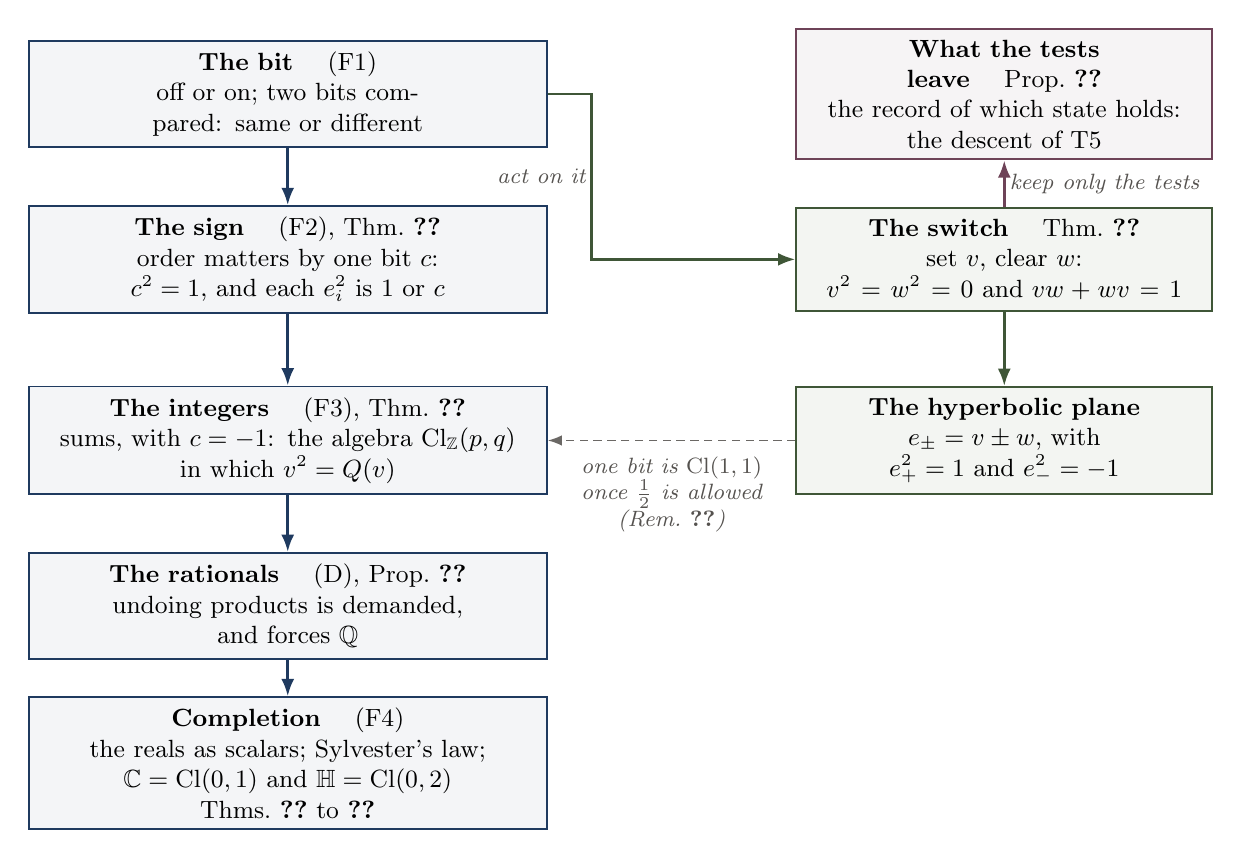
\begin{tikzpicture}[x=1cm, y=1cm, font=\small,
  box/.style={draw, line width=0.7pt, align=center, inner sep=4pt},
  lad/.style={box, draw=TPblue, fill=TPblue!5, text width=6.3cm},
  sw/.style={box, draw=TPgreen!80!black, fill=TPgreen!7, text width=5.0cm},
  pl/.style={box, draw=TPplum, fill=TPplum!6, text width=5.0cm},
  arr/.style={-{Latex[length=2.2mm]}, line width=1.0pt},
  thin/.style={-{Latex[length=1.8mm]}, line width=0.6pt, dash pattern=on 3pt off 2pt},
  lab/.style={font=\footnotesize\itshape, text=TPink!80, inner sep=1.5pt}]
\node[lad] (b) at (0,0) {\textbf{The bit} \quad (F1)\\ off or on; two bits compared: same or different};
\node[lad] (s) at (0,-2.1) {\textbf{The sign} \quad (F2), Thm.~\ref{thm:bitsign}\\ order matters by one bit $c$:\\ \mbox{$c^{2} = 1$}, and each \mbox{$e_{i}^{2}$} is $1$ or $c$};
\node[lad] (z) at (0,-4.4) {\textbf{The integers} \quad (F3), Thm.~\ref{thm:bitclifford}\\ sums, with \mbox{$c = -1$}: the algebra \mbox{$\Cl_{\Z}(p,q)$}\\ in which \mbox{$v^{2} = Q(v)$}};
\node[lad] (q) at (0,-6.5) {\textbf{The rationals} \quad (D), Prop.~\ref{prop:bitdivision}\\ undoing products is demanded,\\ and forces $\Q$};
\node[lad] (r) at (0,-8.5) {\textbf{Completion} \quad (F4)\\ the reals as scalars; Sylvester's law;\\ \mbox{$\C = \Cl(0,1)$} and \mbox{$\HH = \Cl(0,2)$}\\ Thms.~\ref{thm:bitinertia} to \ref{thm:bitfrobenius}};
\node[pl] (pin) at (9.1,0) {\textbf{What the tests leave} \quad Prop.~\ref{prop:pinching}\\ the record of which state holds:\\ the descent of T5};
\node[sw] (sw) at (9.1,-2.1) {\textbf{The switch} \quad Thm.~\ref{thm:switch}\\ set $v$, clear $w$:\\ $v^{2} = w^{2} = 0$ and $vw + wv = 1$};
\node[sw] (hp) at (9.1,-4.4) {\textbf{The hyperbolic plane}\\ \mbox{$e_{\pm} = v \pm w$}, with\\ \mbox{$e_{+}^{2} = 1$} and \mbox{$e_{-}^{2} = -1$}};
\draw[arr, TPblue] (b) -- (s);
\draw[arr, TPblue] (s) -- (z);
\draw[arr, TPblue] (z) -- (q);
\draw[arr, TPblue] (q) -- (r);
\draw[arr, TPgreen!80!black] (b.east) -- ++(0.55,0) |- node[lab, pos=0.25, left] {act on it} (sw.west);
\draw[arr, TPgreen!80!black] (sw) -- (hp);
\draw[arr, TPplum] (sw) -- node[lab, right] {keep only the tests} (pin);
\draw[thin, TPink!70] (hp.west) -- (z.east);
\node[lab, align=center, anchor=north] at ($(hp.west)!0.5!(z.east) + (0,-0.15)$) {one bit is $\Cl(1,1)$\\ once $\tfrac12$ is allowed\\ (Rem.~\ref{rem:twoorders})};
\end{tikzpicture}
\caption{The route of this note. Left, in blue, the ladder: each step forced by the premise or demand named in it and the steps above. Right, in green, the switch: the two operations on one bit and the pair of directions they make. The two columns meet in $\Cl(1,1)$, which is the algebra of one bit once halves are allowed, and keeping only the tests of a register of switches, in plum, leaves the record of which state holds and nothing that changes it.}
\label{fig:route}
\end{figure}

\section{The bit and its repetition}\label{sec:repetition}

\begin{premise}[F1, the bit]
There is a single distinction with two states, \emph{off} (nothing) and \emph{on} (something). Distinctions are combined by comparison: two states that agree give off, two that differ give on, so that making a distinction and making it again returns to nothing. Distinctions can be repeated independently: for $n$ of them, a \emph{configuration} is the set $S \subseteq \{1, \dots, n\}$ of those that are on, and configurations are compared distinction by distinction, which is the symmetric difference
\[
S \mathbin{\triangle} T \;=\; (S \cup T) \setminus (S \cap T) .
\]
\end{premise}

No coefficient ring has been used: counting serves only to name the configurations. Counting the configurations, when numbers are later available, gives $2^{n}$ of them, of which $\binom{n}{k}$ have exactly $k$ distinctions on: the dimension count and the grade count of the primer \cite[Section 3]{ButlerT0}. In later language the configurations form the vector space $\F_{2}^{n}$ over the field with two elements, and that name is used below as a label only.

What the bit does not contain is as important. It has no sign, since a distinction cannot be told from its reversal. It has no order, since comparison is symmetric. It has no magnitude and no geometry.

\section{Order, and the arrival of the sign}\label{sec:sign}

The second premise says only that the order in which two different distinctions are made can matter, and that when it does it matters by a single sign. Formally:

\begin{premise}[F2, minimal non-commutativity]
Grant (F1), with $n \geq 1$ distinctions. There is a group $G$, generated by \emph{directions} $e_{1}, \dots, e_{n}$ and one further element $c$, such that:
\begin{enumerate}
\item[(F2a)] $c$ commutes with every element of $G$, and $c^{2} = 1$;
\item[(F2b)] modulo $c$ the group is the configurations: $G/\langle c \rangle$ is commutative, each of its elements is its own inverse, and $S \mapsto e_{S}\langle c\rangle$ is a bijection from the configurations, carrying $\triangle$ to the product, where $e_{S}$ is the product of the $e_{i}$, $i \in S$, in increasing order;
\item[(F2c)] $c \neq 1$, and for $i \neq j$
\[
e_{i}\,e_{j} \;=\; c\,e_{j}\,e_{i} .
\]
\end{enumerate}
\end{premise}

In words: the order in which two different distinctions are made now matters, and it matters by exactly one bit, the element $c$. This is the sense in which the non-commutativity is called minimal: every pair of different directions fails to commute by the same single element. The premise does not say which directions square to $c$ and which to $1$; every choice is allowed, and Theorem \ref{thm:bitsign}(v) shows that every choice occurs.

\begin{theorem}[The sign and the blades]\label{thm:bitsign}
Grant \textup{(F1)} and \textup{(F2)}.
\begin{enumerate}
\item[(i)] For $n \geq 2$ the clause $c^{2} = 1$ of \textup{(F2a)} follows from \textup{(F2c)}.
\item[(ii)] Each $e_{i}^{2}$ is $1$ or $c$. Write $N$ for the set of $i$ with $e_{i}^{2} = c$.
\item[(iii)] Every element of $G$ is $e_{S}$ or $c\,e_{S}$ for exactly one configuration $S$, and
\[
e_{S}\,e_{T} \;=\; c^{\,f(S,T)}\,e_{S \triangle T}, \qquad
f(S,T) \;=\; \#\{(i,j) \in S \times T : i > j\} \;+\; \#(S \cap T \cap N) .
\]
\item[(iv)] With exponents read modulo $2$,
\[
e_{S}^{2} \;=\; c^{\,q(S)}, \qquad e_{S}\,e_{T} \;=\; c^{\,b(S,T)}\,e_{T}\,e_{S},
\]
\[
q(S) \;=\; \binom{|S|}{2} + |S \cap N|, \qquad b(S,T) \;=\; |S|\,|T| + |S \cap T| ,
\]
and $q(S \mathbin{\triangle} T) = q(S) + q(T) + b(S,T)$.
\item[(v)] \textup{(Existence.)} For every $n \geq 1$ and every set $N \subseteq \{1, \dots, n\}$ there is a group $G$ as in \textup{(F2)} in which $e_{i}^{2} = c$ exactly for $i \in N$.
\end{enumerate}
\end{theorem}

\noindent\emph{How the proof goes.} Any product of directions can be put in increasing order, each exchange of two different directions costing one $c$ and each repeated direction being replaced by its square; counting the costs gives $f$, and part (v) builds the group from that same rule. Example~\ref{ex:twobits} is the case $n = 2$. The proof is in Appendix~\ref{prf:thm:bitsign}.

So three things have appeared before any addition and before any coefficient ring: a sign (the element $c$, which will act as $-1$), a signature (the set $N$, which is a choice), and, as soon as $n \geq 2$, an element squaring to the sign whatever the signature: either some $e_{i}$ does, or two directions outside $N$ have $q(\{i,j\}) = 1$, so that $e_{i}e_{j}$ squares to $c$ (the unit bivector of \cite[Example 2.1]{ButlerT0}). The functions $q$ and $b$ are a quadratic form on the configurations and its polar form: the signature is a quadratic form over the bit.

\begin{example}[Two bits]\label{ex:twobits}
Take $n = 2$ with neither direction in $N$, so that $e_{1}^{2} = e_{2}^{2} = 1$. Premise (F2c) gives $e_{2}e_{1} = c\,e_{1}e_{2}$, and so
\[
(e_{1}e_{2})^{2} \;=\; e_{1}\,(e_{2}e_{1})\,e_{2} \;=\; c\,e_{1}e_{1}\,e_{2}e_{2} \;=\; c .
\]
In Theorem~\ref{thm:bitsign}(iii) this is $f(\{1,2\},\{1,2\}) = 1$: one pair $(2,1)$ with $2 > 1$, and nothing in $N$. So with two bits, and no sign put on either direction, the product of the two directions squares to the sign. When (F3) reads $c$ as $-1$ this is the unit bivector of the primer, the element that will play the complex unit. The whole multiplication table, row times column, is
\[
\begin{array}{c|cccc}
 & 1 & e_{1} & e_{2} & e_{1}e_{2} \\ \hline
1 & 1 & e_{1} & e_{2} & e_{1}e_{2} \\
e_{1} & e_{1} & 1 & e_{1}e_{2} & e_{2} \\
e_{2} & e_{2} & c\,e_{1}e_{2} & 1 & c\,e_{1} \\
e_{1}e_{2} & e_{1}e_{2} & c\,e_{2} & e_{1} & c
\end{array}
\]
and each $c$ in it counts one exchange of $e_{2}$ past $e_{1}$.
\end{example}


\section{Superposition, and the one rule as a theorem}\label{sec:superposition}

The third premise lets elements be added, which brings in the integers as counts, and reads the sign as $-1$. Formally:

\begin{premise}[F3, superposition over the integers]
Grant (F2). Elements of $G$ can be added, and the sign bit acts as $-1$. With $\Z[G]$ the formal sums of elements of $G$ with integer coefficients, multiplied through the product of $G$, the algebra of the foundation is the quotient
\[
A \;=\; \Z[G]\,/\,(c + 1) .
\]
\end{premise}

The integers enter here, as counts of how many times a configuration is added, and $-1$ enters as the image of $c$. For a commutative ring $R$ write $A_{R} = R[G]/(c+1)$ for the same construction with coefficients in $R$, and for $x \in R^{n}$ put
\[
Q(x) \;=\; \sum_{i \notin N} x_{i}^{2} \;-\; \sum_{i \in N} x_{i}^{2} .
\]

\begin{theorem}[The integer algebra is the Clifford algebra]\label{thm:bitclifford}
Grant \textup{(F1)} to \textup{(F3)}, and let $R$ be a commutative ring.
\begin{enumerate}
\item[(i)] $A_{R}$ is a free $R$-module with basis the $2^{n}$ elements $e_{S}$, and
$e_{S}\,e_{T} = (-1)^{f(S,T)}\,e_{S \triangle T}$.
\item[(ii)] \textup{(The one rule.)} For $v = \sum_{i} x_{i}e_{i}$ with $x \in R^{n}$,
\[
v^{2} \;=\; Q(x) .
\]
\item[(iii)] \textup{(Universal property.)} Let $B$ be an associative $R$-algebra with unit and $\phi : R^{n} \to B$ an $R$-linear map with $\phi(x)^{2} = Q(x)\,1$ for all $x$. Then there is exactly one homomorphism of $R$-algebras $\Phi : A_{R} \to B$ with $\Phi(\sum_{i} x_{i}e_{i}) = \phi(x)$.
\end{enumerate}
So $A_{R}$ is the Clifford algebra $\Cl_{R}(p,q)$ of the form $Q$, with $q = |N|$ and $p = n - q$; in particular $A = \Cl_{\Z}(p,q)$, and $A_{\R}$ is the algebra $\Cl(p,q)$ of the primer \cite[Sections 2 to 4]{ButlerT0} with the $e_{S}$ its basis blades.
\end{theorem}

\noindent\emph{How the proof goes.} Setting $c = -1$ leaves the $2^{n}$ blades as a basis, and in $v^{2}$ the cross terms cancel in pairs because different directions anticommute, which leaves $Q$. Part (iii) follows by running the same sorting in any algebra whose vectors square by $Q$. Example~\ref{ex:onerule} is the case $n = 2$. The proof is in Appendix~\ref{prf:thm:bitclifford}.

The primer \cite[Section 2]{ButlerT0} takes $v^{2} = Q(v)$ as the one rule from which the geometric product is generated. From the bit it is not a rule but a consequence: it is what one bit of non-commutativity and the freedom to add leave behind. The construction of a Clifford algebra as a group algebra twisted by a sign is known \cite{AlbuquerqueMajid2002}; what is added here is its reading as the second and third steps from a single distinction.

\begin{example}[The one rule by hand]\label{ex:onerule}
Take $n = 2$ with $N = \{2\}$, so that after (F3) $e_{1}^{2} = 1$, $e_{2}^{2} = -1$ and $e_{1}e_{2} = -e_{2}e_{1}$. For integers $a$, $b$ and $v = a e_{1} + b e_{2}$,
\[
v^{2} \;=\; a^{2}e_{1}^{2} + ab\,(e_{1}e_{2} + e_{2}e_{1}) + b^{2}e_{2}^{2} \;=\; a^{2} - b^{2} \;=\; Q(v) .
\]
The cross terms cancel because the two directions anticommute, and the minus sign is the choice $N = \{2\}$. Nothing about $v^{2}$ was assumed: the one rule came out. With $a = b = 1$ the vector $e_{1} + e_{2}$ squares to $0$, a null vector over the integers.
\end{example}


\section{Division, and the rationals}\label{sec:division}

The next step is a demand rather than a premise about the bit. It is the primer's requirement \cite[Section 2]{ButlerT0} that the product can be undone, asked of the integer vectors that can be inverted at all:

\begin{premise}[D, division]
Every integer vector $v$ with $Q(v) \neq 0$ has an inverse.
\end{premise}

\begin{proposition}[Division produces the rationals]\label{prop:bitdivision}
Let $R$ be a commutative ring. Every integer vector $v = \sum_{i} a_{i}e_{i}$ with $Q(v) \neq 0$ in $\Z$ is invertible in $A_{R}$ if and only if every nonzero integer is invertible in $R$.
\end{proposition}

\noindent\emph{How the proof goes.} A vector with $Q(v) \neq 0$ has the inverse $v/Q(v)$; conversely the vector $m e_{1}$ shows that each nonzero integer $m$ must be invertible. Example~\ref{ex:half} is the smallest case. The proof is in Appendix~\ref{prf:prop:bitdivision}.

Every nonzero ring in which every nonzero integer is invertible contains exactly one copy of $\Q$. So the rational numbers are what the demand (D) forces on the coefficients, and nothing less will do: every fraction $a/m$ is the product $(a e_{1})(m e_{1})^{-1}$ of an integer vector and the inverse of one. Premise (F4) below posits a field containing $\Q$ in any case; what (D) and Proposition~\ref{prop:bitdivision} add is that nothing smaller than $\Q$ will do once division is asked for.

Division does not remove everything. When $p \geq 1$ and $q \geq 1$ the null vectors of the primer \cite[Section 4]{ButlerT0} are there over $\Z$ and remain over $\Q$, for instance $e_{i} + e_{j}$ with $i \notin N$ and $j \in N$, and no extension of the coefficients inverts them. That is where T1 begins.

\begin{example}[A vector that needs a half]\label{ex:half}
With $n = 2$ and $N$ empty, the integer vector $v = e_{1} + e_{2}$ has $v^{2} = 2$, so
\[
v \cdot \tfrac12\,v \;=\; 1 ,
\]
and its inverse $\tfrac12(e_{1} + e_{2})$ exists over $\Q$ but not over $\Z$. In $\Cl(1,1)$, by contrast, the null vector $e_{1} + e_{2}$ of Example~\ref{ex:onerule} has no inverse over any nonzero coefficient ring: if $vu = 1$ then $v = v(vu) = v^{2}u = 0$, which is false.
\end{example}


\section{Completion, and the number systems inside}\label{sec:completion}

The fourth and last premise asks for limits. Formally:

\begin{premise}[F4, completion]
The coefficients are extended from $\Q$ to a complete ordered field $\R$: an ordered field in which every nonempty set that is bounded above has a least upper bound.
\end{premise}

This is the one step that is not algebraic, and it is the last premise. What it gives is proved here in three stages: square roots, and with them the classification of quadratic forms by their signs; roots of polynomials; and the list of the algebras in which division never fails. The results are classical \cite{Lam2005, Ebbinghaus1991}; the proofs are written out so that the step to the real numbers rests on (F4) and on nothing else.

Some vocabulary first. Let $F$ be an ordered field. A \emph{quadratic space} over $F$ is a finite-dimensional vector space $V$ with a map $Q : V \to F$ such that $Q(\lambda v) = \lambda^{2}Q(v)$ and
\[
B(u, v) \;=\; \tfrac12\bigl(Q(u + v) - Q(u) - Q(v)\bigr)
\]
is bilinear; then $Q(v) = B(v, v)$. Vectors $u, v$ are \emph{orthogonal} when $B(u,v) = 0$; in any algebra in which $v^{2} = Q(v)$, expanding $(u+v)^{2}$ gives $uv + vu = 2B(u,v)$, so orthogonal vectors are exactly those that anticommute. An \emph{isometry} is a linear bijection that preserves $Q$. The field $F$ is \emph{Euclidean} when every positive element is a square (and $0 = 0^{2}$, so then every element that is not negative is one). For $a \in F$, $|a|$ is $a$ or $-a$, whichever is not negative; one checks from the rules of the order, case by case on the signs, that $|ab| = |a|\,|b|$ and $|a + b| \leq |a| + |b|$. Finally, in an ordered field $1 = 1^{2} > 0$, so $m \cdot 1 > 0$ for every positive integer $m$: the field contains $\Q$, it is infinite, and division by $2$ is always possible.

\begin{theorem}[Square roots and the law of inertia]\label{thm:bitinertia}
Let $F$ be an ordered field and $(V, Q)$ a quadratic space over $F$ of dimension $n$.
\begin{enumerate}
\item[(i)] If $F$ is complete, then $F$ is Euclidean.
\item[(ii)] $V$ has a basis of mutually orthogonal vectors. If $F$ is Euclidean, it has one in which every $Q(u_{i})$ is $1$, $-1$ or $0$.
\item[(iii)] \textup{(Sylvester's law of inertia.)} The numbers $p$, $q$, $r$ of vectors with $Q > 0$, $Q < 0$, $Q = 0$ are the same in every orthogonal basis: $p$ and $q$ are the largest dimensions of subspaces on whose nonzero vectors $Q$ is positive, respectively negative, and $r$ is the dimension of the radical.
\item[(iv)] If $F$ is Euclidean, two quadratic spaces over $F$ are isometric exactly when they have the same $(p, q, r)$. If moreover $r = 0$ and $n \geq 1$, the algebra $A_{F}$ of Theorem \ref{thm:bitclifford} with $|N| = q$ (which exists by Theorem \ref{thm:bitsign}(v)), together with an isometry $V \to F^{n}$, has the universal property of Theorem \ref{thm:bitclifford}(iii) for $(V, Q)$.
\end{enumerate}
\end{theorem}

\noindent\emph{How the proof goes.} Square roots come from the least upper bound of the numbers whose square is at most $a$; orthogonal bases come by induction, splitting off one vector of nonzero square at a time; the counts are then compared directly. These are the classical arguments, written out so that they use (F4) and nothing more. The proof is in Appendix~\ref{prf:thm:bitinertia}.

So over $\R$ a quadratic form is known by three counts, and when it is nondegenerate its algebra is one of the algebras $A_{\R} = \Cl(p,q)$ the bit produced. Part (iii) used only the order and part (ii) only square roots of positive numbers. Over $\Q$, where those roots are missing, a direction carries more than a sign: its square is fixed only up to multiplication by a nonzero rational square, so that $x^{2}$ and $2x^{2}$ are different forms with the same counts.

The second stage needs two standard tools of polynomial algebra, proved here for completeness.

\begin{lemma}[Two tools]\label{lem:bitpoly}
Let $K$ be a field.
\begin{enumerate}
\item[(a)] For every nonconstant polynomial $p$ over $K$ there is a field $L \supseteq K$ over which $p$ is a product of factors of degree $1$.
\item[(b)] A polynomial over $K$ in variables $r_{1}, \dots, r_{n}$ that is unchanged by every permutation of the variables is a polynomial over $K$ in the elementary symmetric polynomials
\[
\sigma_{k} \;=\; \sum_{i_{1} < \dots < i_{k}} r_{i_{1}} \cdots r_{i_{k}}, \qquad 1 \leq k \leq n .
\]
\end{enumerate}
\end{lemma}

\noindent\emph{How the proof goes.} Both are classical: (a) by adjoining a root of an irreducible factor and inducting on the degree, (b) by removing the leading term again and again. The proof is in Appendix~\ref{prf:lem:bitpoly}.

Write $\C$ for the algebra $A_{\R}$ with one direction $e$ of square $-1$, that is $\Cl(0,1)$: its elements are $z = a + be$ with $a, b \in \R$. It is commutative, and with $\bar{z} = a - be$,
\[
z\,\bar{z} \;=\; a^{2} + b^{2} ,
\]
which is positive unless $z = 0$. So every nonzero $z$ has the inverse $\bar{z}/(z\bar{z})$: $\C$ is a field, the map $z \mapsto \bar{z}$ respects sums and products, and the elements it fixes are those of $\R$.

\begin{theorem}[Real polynomials have their roots in $\Cl(0,1)$]\label{thm:bitroots}
Let $\R$ be a complete ordered field.
\begin{enumerate}
\item[(i)] Every polynomial over $\R$ of odd degree has a root in $\R$.
\item[(ii)] Every element of $\C$ is a square in $\C$.
\item[(iii)] Every nonconstant polynomial over $\R$ has a root in $\C$.
\item[(iv)] A polynomial that is irreducible over $\R$ has degree $1$ or $2$.
\end{enumerate}
\end{theorem}

\noindent\emph{How the proof goes.} (i) uses the least upper bound, (ii) writes the square roots down, and (iii) is Laplace's argument, an induction on the power of $2$ in the degree that uses Lemma~\ref{lem:bitpoly}; (iv) follows from (iii). Example~\ref{ex:roots} shows a pair of roots. The proof is in Appendix~\ref{prf:thm:bitroots}.

This is the fundamental theorem of algebra, by Laplace's argument \cite{Ebbinghaus1991}. (The same holds for a nonconstant polynomial $f$ with coefficients in $\C$: the product of $f$ and the polynomial with the conjugate coefficients has real coefficients, so it has a root $z \in \C$, and then $f(z) = 0$ or $f(\bar{z}) = 0$.) The theorem places the complex numbers: they are not adjoined to the real numbers from outside but are the algebra of one direction of square $-1$, and that algebra already holds the roots of every real polynomial. Completeness was used twice only, for square roots and for (i).

\begin{theorem}[Frobenius: where division never fails]\label{thm:bitfrobenius}
Let $\R$ be a complete ordered field and $D \neq 0$ an associative $\R$-algebra with unit, of finite dimension, in which a product of nonzero elements is never zero. Then $D$ is isomorphic to exactly one of
\[
\R, \qquad \C = \Cl(0,1), \qquad \HH = \Cl(0,2) ,
\]
the algebras of no direction, one direction and two directions of square $-1$.
Conversely, in each of these three a product of nonzero elements is never zero.
\end{theorem}

\noindent\emph{How the proof goes.} Every element satisfies a real polynomial of degree at most $2$; the elements whose square is real and not positive form a subspace $V$, on which $-x^{2}$ is a positive form; $V$ has dimension $0$, $1$ or $3$, and in the last case the third direction is the product of the first two (Palais's argument). The proof is in Appendix~\ref{prf:thm:bitfrobenius}.

The theorem is due to Frobenius \cite{Frobenius1878}; the proof through the subspace of elements with non-positive square follows Palais \cite{Palais1968}. Read in the algebra, it says that the only directions that can be added without ever losing division are at most two, both of square $-1$: a third must be the product of the first two.

With these three theorems the order of the textbooks is reversed. The real numbers are the scalars of the completed algebra; the complex numbers and the quaternions are two of its smallest members; and by the classification of the real Clifford algebras (imported from \cite[Theorem 9.3]{ButlerT0}, where its induction is cited and not repeated, and used here in this sentence only, in no proof), every other $\Cl(p,q)$ is a matrix algebra over one of the three, or a sum of two. The number systems in common use sit inside the algebra the bit generates.

\begin{example}[Roots in $\Cl(0,1)$, and Hamilton's relations]\label{ex:roots}
The polynomial $x^{2} - 2x + 5$ has no real root, and in $\C = \Cl(0,1)$, with $e^{2} = -1$, it has the roots $1 \pm 2e$:
\[
(1 + 2e)^{2} - 2(1 + 2e) + 5 \;=\; (1 + 4e - 4) - 2 - 4e + 5 \;=\; 0 ,
\]
and likewise for $1 - 2e$. In $\HH = \Cl(0,2)$ put $i = e_{1}$, $j = e_{2}$ and $k = e_{1}e_{2}$. Then
\[
i^{2} = j^{2} = k^{2} = -1, \qquad ij = k = -ji ,
\]
since $k^{2} = e_{1}e_{2}e_{1}e_{2} = -e_{1}e_{1}e_{2}e_{2} = -1$: these are Hamilton's relations. A third direction of square $-1$ breaks division, as Theorem~\ref{thm:bitfrobenius} says it must. In $\Cl(0,3)$ the element $u = e_{1}e_{2}e_{3}$ has $u^{2} = 1$, and so
\[
(1 - u)(1 + u) \;=\; 1 - u^{2} \;=\; 0
\]
with both factors nonzero.
\end{example}


Two remarks on what (F4) is needed for. Theorems \ref{thm:bitroots} and \ref{thm:bitfrobenius} use completeness only through square roots of positive numbers and roots of polynomials of odd degree, so they hold over every ordered field with those two properties, for example the real algebraic numbers. Completeness itself is needed for limits, such as the half-angle rotor of \cite[Example 6.1]{ButlerT0}, which needs completeness to be defined for every angle.

One family is not reached by any finite step. The commutation relation of a boson, $ab - ba = 1$, has no solution in a nonzero finite-dimensional real algebra: acting on the algebra by left multiplication, $ab - ba$ has trace $0$ and $1$ has trace the dimension. Whether such relations arise as a limit on the infinite tower of T3 \cite{ButlerT3} lies outside this note.

\section{The switch: what a bit does}\label{sec:switch}

The ladder above treats a distinction as something that can be made and made again, and the direction $e_{i}$ is that operation. A bit can also be acted on in a less symmetric way: it can be \emph{set} and it can be \emph{cleared}. This section shows that those two operations are exactly a hyperbolic pair, that they need no fractions, and that the integer algebra of the ladder does not contain them.

\begin{definition}[Bit, set, clear, switch]\label{def:switch}
Let $R$ be a commutative ring. A \emph{bit over $R$} is the free module
\[
M \;=\; R\,s_{\mathrm{off}} \oplus R\,s_{\mathrm{on}}
\]
on the two states. \emph{Set} is the $R$-linear map $v$ and \emph{clear} the $R$-linear map $w$ with
\[
v\,s_{\mathrm{off}} = s_{\mathrm{on}}, \quad v\,s_{\mathrm{on}} = 0, \qquad\qquad w\,s_{\mathrm{on}} = s_{\mathrm{off}}, \quad w\,s_{\mathrm{off}} = 0 .
\]
A \emph{switch} in an associative ring with unit is a pair $(a, b)$ with
\[
a^{2} = 0, \qquad b^{2} = 0, \qquad ab + ba = 1 .
\]
\end{definition}

\begin{theorem}[The switch generates the hyperbolic plane]\label{thm:switch}
Let $M$ be a bit over a commutative ring $R$, with set $v$ and clear $w$.
\begin{enumerate}
\item[(i)] $(v, w)$ is a switch. The products $vw$ and $wv$ are idempotent, $vw + wv = 1$ and $vw \cdot wv = wv \cdot vw = 0$; $vw$ fixes $s_{\mathrm{on}}$ and kills $s_{\mathrm{off}}$, and $wv$ does the reverse.
\item[(ii)] The $R$-algebra generated by $v$ and $w$ is all of $\mathrm{End}_{R}(M)$, which is free with basis $1, v, w, vw$.
\item[(iii)] For $x = \alpha v + \beta w$ with $\alpha, \beta \in R$,
\[
x^{2} \;=\; \alpha\beta .
\]
With $L = Rv \oplus Rw$ and $Q(x) = \alpha\beta$, the algebra $\mathrm{End}_{R}(M)$ has the universal property of Theorem \ref{thm:bitclifford}(iii) for $(L, Q)$: it is the Clifford algebra of the hyperbolic plane, over every $R$.
\item[(iv)] The elements $e_{+} = v + w$ and $e_{-} = v - w$ satisfy
\[
e_{+}^{2} = 1, \qquad e_{-}^{2} = -1, \qquad e_{+}e_{-} = -e_{-}e_{+} = wv - vw .
\]
$e_{+}$ exchanges the two states, and $e_{+}e_{-}$ is $+1$ on $s_{\mathrm{off}}$ and $-1$ on $s_{\mathrm{on}}$.
\end{enumerate}
\end{theorem}

\noindent\emph{How the proof goes.} Everything is read off from what $v$ and $w$ do to the two states. Example~\ref{ex:tables} shows each identity as a two-by-two table. The proof is in Appendix~\ref{prf:thm:switch}.

Nothing in the statement or the proof divides by $2$, and no sign was put in: the relations of a single fermionic mode, $v^{2} = w^{2} = 0$ and $vw + wv = 1$ \cite{JordanWigner1928}, are the relations of setting and clearing a bit. ``It cannot be set twice'' is $v^{2} = 0$, and ``it is either on or off'' is $vw + wv = 1$. That the Clifford algebra of the hyperbolic plane is the $2 \times 2$ matrix ring over every commutative ring is classical \cite{Bass1974, Knus1991}. The primer's Example 4.1 \cite{ButlerT0} met the same pair from the other side, as $\tfrac12(e_{1} \pm e_{2})$, where the $\tfrac12$ was needed; part (iv) is that example read backwards, and it produces the two directions of squares $+1$ and $-1$ from the switch without any fraction.

\begin{example}[The switch as two-by-two tables]\label{ex:tables}
In the basis $s_{\mathrm{off}}, s_{\mathrm{on}}$, each column giving the image of a state,
\[
v = \begin{pmatrix} 0 & 0 \\ 1 & 0 \end{pmatrix}, \qquad
w = \begin{pmatrix} 0 & 1 \\ 0 & 0 \end{pmatrix}, \qquad
vw = \begin{pmatrix} 0 & 0 \\ 0 & 1 \end{pmatrix}, \qquad
wv = \begin{pmatrix} 1 & 0 \\ 0 & 0 \end{pmatrix} .
\]
So $v^{2} = w^{2} = 0$ (setting twice gives nothing), $vw$ is the test for on and $wv$ the test for off, and $vw + wv = 1$. The sum and the difference are
\[
e_{+} = v + w = \begin{pmatrix} 0 & 1 \\ 1 & 0 \end{pmatrix}, \qquad
e_{-} = v - w = \begin{pmatrix} 0 & -1 \\ 1 & 0 \end{pmatrix},
\]
with $e_{+}^{2} = 1$ (exchanging the states twice changes nothing), $e_{-}^{2} = -1$, and $e_{+}e_{-} = \begin{pmatrix} 1 & 0 \\ 0 & -1 \end{pmatrix}$. No entry is a fraction.
\end{example}


The next result says that this is not one way of putting directions on a bit among many.

\begin{proposition}[Planes of directions on two states]\label{prop:planes}
Let $F$ be a field in which $2 \neq 0$, $E$ the algebra of linear maps of $F^{2}$, and $E_{0}$ the maps of trace zero.
\begin{enumerate}
\item[(i)] If $V \subseteq E$ is a subspace of dimension at least $2$ in which every element squares to a scalar, then $V \subseteq E_{0}$. On $E_{0}$, $x^{2} = -\det x =: Q(x)$, and over an ordered field $Q$ has signature $(2,1)$, that is $(p,q,r) = (2,1,0)$ in the sense of Theorem \ref{thm:bitinertia}.
\item[(ii)] Let $V \subseteq E_{0}$ be a plane. The nonzero elements of $V$ with square zero form two lines exactly when $V$ is spanned by a switch, one line exactly when $Q$ restricted to $V$ is degenerate, and no line otherwise.
\item[(iii)] Over an ordered field the signature of $Q$ on $V$ is $(2,0)$, $(1,1)$, or degenerate with one positive direction, and no other. If every positive element of $F$ is a square, $V$ is spanned by a switch exactly when the signature is $(1,1)$.
\item[(iv)] $V$ generates $E$ when $Q$ is nondegenerate on $V$, and a subalgebra of dimension $3$ when it is degenerate.
\item[(v)] Sending a switch $(a, b)$ to the pair of lines $\{\ker a, \ker b\}$ is a bijection from the planes spanned by a switch to the unordered pairs of distinct lines of $F^{2}$. Any two such planes are conjugate by an invertible map.
\end{enumerate}
\end{proposition}

\noindent\emph{How the proof goes.} Every $2 \times 2$ matrix satisfies $x^{2} = (\operatorname{tr} x)\,x - \det x$, so a square that is a scalar forces trace zero; the rest is a computation on the maps of trace zero. The proof is in Appendix~\ref{prf:prop:planes}.

So on a system with two states, over the real numbers, a plane of directions that generates all the operations is either of signature $(2,0)$, which contains no operation of square zero, or it is a hyperbolic plane spanned by a switch, and the hyperbolic planes are exactly the choices of what the two states are. The pair of directions with squares $+1$ and $-1$ is the pair that goes with a bit that can be set and cleared.

\begin{theorem}[The integer algebra of the ladder contains no switch]\label{thm:nobit}
Let $\Cl_{R}(p,q) = A_{R}$ be the algebra of Theorem \ref{thm:bitclifford}, with $n = p + q \geq 1$ and the directions ordered so that $N = \{p+1, \dots, n\}$.
\begin{enumerate}
\item[(i)] $\Cl_{\Z}(p,q)$ has no idempotent other than $0$ and $1$.
\item[(ii)] If $ab + ba = 1$ for some $a, b \in \Cl_{R}(p,q)$, then $2$ is invertible in $R$. In particular $\Cl_{\Z}(p,q)$ contains no switch.
\item[(iii)] If $2$ is invertible in $R$ and $p, q \geq 1$, then $\tfrac12(e_{1} + e_{p+1})$, $\tfrac12(e_{1} - e_{p+1})$ is a switch.
\end{enumerate}
\end{theorem}




\noindent\emph{How the proof goes.} Modulo $2$ the algebra is commutative and every blade squares to $1$. So there the square of an element is a scalar, the sum of its coefficients, and an idempotent is $0$ or $1$ modulo $2$, which a $2$-adic argument lifts to (i); and $ab + ba = 2ab$ vanishes, so $ab + ba = 1$ is possible only if $2$ is invertible, which is (ii). Part (iii) is a two-line computation. Example~\ref{ex:halves} shows the case $p = q = 1$ by hand. The proof is in Appendix~\ref{prf:thm:nobit}.

\begin{example}[The ladder needs halves to set a bit]\label{ex:halves}
Send the two directions of $\Cl_{\Z}(1,1)$ to $e_{+}$ and $e_{-}$ of Example~\ref{ex:tables}. The element $\alpha + \beta e_{1} + \gamma e_{2} + \delta e_{1}e_{2}$, with integer coefficients, becomes
\[
\begin{pmatrix} \alpha + \delta & \beta - \gamma \\ \beta + \gamma & \alpha - \delta \end{pmatrix} .
\]
The exchange $e_{+}$ is there, with $\beta = 1$. Setting the bit needs $\beta + \gamma = 1$ and $\beta - \gamma = 0$, so $\beta = \gamma = \tfrac12$; the test for on needs $\alpha = \tfrac12$ and $\delta = -\tfrac12$. Over the integers the ladder can exchange the two states but can neither set the bit nor test it. With halves it can do both, and $\tfrac12(e_{1} + e_{2})$, $\tfrac12(e_{1} - e_{2})$ is the switch of Theorem~\ref{thm:nobit}(iii).
\end{example}

\begin{remark}[Two orders of construction]\label{rem:twoorders}
Theorems \ref{thm:switch} and \ref{thm:nobit} separate two ways of building on the bit, which agree as soon as $2$ is invertible and differ before.

In the ladder of (F1) to (F3) the direction is the reversible operation, the one that is undone, up to the sign, by repeating it. Over the integers this algebra can exchange the two states, but by Theorem \ref{thm:nobit}(i) it contains no test for which state holds: the tests $vw$ and $wv$ are idempotents. They arrive only once $2$ is inverted, which the step to $\Q$ of Proposition \ref{prop:bitdivision} does.

Starting instead from the switch, the tests and the two irreversible operations are there at once, over the integers, and the reversible directions are their sum and difference. For one switch the comparison is exact. Send the two directions of $\Cl_{\Z}(1,1)$ to $e_{+} = v + w$ and $e_{-} = v - w$, as in Theorem \ref{thm:switch}(iv). The element $\alpha + \beta e_{+} + \gamma e_{-} + \delta e_{+}e_{-}$ then has, in the basis of the states, the diagonal entries $\alpha + \delta$, $\alpha - \delta$ and the off-diagonal entries $\beta - \gamma$, $\beta + \gamma$. So the image of $\Cl_{\Z}(1,1)$ is the integer matrices whose diagonal entries have the same parity and whose off-diagonal entries have the same parity: a subring of index $4$ in $\mathrm{End}_{\Z}(M)$.

Hence the map $\Cl_{R}(1,1) \to \mathrm{End}_{R}(M)$ with $e_{1} \mapsto e_{+}$ and $e_{2} \mapsto e_{-}$ is an isomorphism exactly when $2$ is invertible in $R$. If it is, the matrix above can be solved for $\alpha, \beta, \gamma, \delta$; if the map is an isomorphism, $\Cl_{R}(1,1)$ contains a copy of the switch $(v, w)$, and Theorem~\ref{thm:nobit}(ii) makes $2$ invertible.

Which order the foundation should take is not settled here. The premises (F1) to (F4) are stated as they stand, and the switch is recorded beside them. Proposition \ref{prop:pinching} below gives the map that joins the two.

\emph{Status.} The index and the isomorphism are proved. Which order the foundation takes is a choice, and it is open.
\end{remark}

\begin{remark}[Argued: the algebra of physics]\label{rem:argued}
\emph{Status: argued, not proved, and not used anywhere in the series' proofs.} The reading is that geometric algebra is the natural language of physics because it is a minimal structure that independent distinctions carry once their order may matter, minimal in the sense of (F2): one central sign, the same for every pair of distinctions, and that the numbers in common use are parts of that structure and not its foundation.

The evidence is that the structures physics found one at a time appear early on the ladder: the two-to-one covering of rotations by rotors \cite[Example 6.1]{ButlerT0}; a plane of square $-1$ in the place of the complex unit; $\Cl(3,0)$ and $\Cl(1,3)$ for spin and for the Dirac theory \cite{Hestenes1966, Hestenes2003}; a signature with both signs for spacetime; and, by Theorem \ref{thm:switch}, the relations of a fermion as the relations of setting and clearing a bit. The difference from the classical development of geometric algebra \cite{HestenesSobczyk1984} is the order: there the real numbers are given and the geometric product is built over them; here the distinction is given and the numbers follow.

The objections belong with the reading. The premises are chosen, and the derivation shows only what follows once they are granted. Every finite-dimensional associative real algebra embeds in a matrix algebra, so containing the number systems is cheap; what the algebra adds is the grading and the geometric meaning. Anything stated in geometric algebra can be restated with matrices or tensors. Bosons and the continuum each rest on a premise. A fundamental role for a non-associative structure such as the octonions would show that the ladder misses something essential. Wheeler, cited in Section~\ref{sec:bit} for ``it from bit'', rejects the continuum that (F4) posits. And the premises were chosen knowing where they lead: (F2) and (F3) are the standard presentation of a Clifford algebra by generators and relations, read from the bit, so arriving at geometric algebra is by construction; the evidence was assembled knowing the physics it had to cover, which makes it weaker than a prediction.
\end{remark}

\section{What the tests leave of a switch}\label{sec:tests}

Remark \ref{rem:twoorders} set the ladder and the switch side by side. One map joins them. Keep the tests of $n$ switches and discard everything that changes a state. What is left is the algebra of functions on the configurations of premise (F1), and when $2 \neq 0$ it carries their comparison.

\begin{definition}[Register, tests, parities, pinching]\label{def:register}
Let $R$ be a commutative ring and $n \geq 1$. The \emph{register} $M_{n}$ is the free $R$-module on the configurations $S \subseteq \{1, \dots, n\}$ of (F1), with basis $s_{S}$. For each $i$, \emph{set} and \emph{clear} are the $R$-linear maps
\[
v_{i}\,s_{S} \;=\;
\begin{cases}
\sigma_{i}(S)\,s_{S \cup \{i\}} & i \notin S \\
0 & i \in S
\end{cases}
\qquad\qquad
w_{i}\,s_{S} \;=\;
\begin{cases}
\sigma_{i}(S)\,s_{S \setminus \{i\}} & i \in S \\
0 & i \notin S
\end{cases}
\]
where either $\sigma_{i}(S) = 1$ throughout (the \emph{plain} register), or
\[
\sigma_{i}(S) \;=\; (-1)^{\#\{j \in S \,:\, j < i\}}
\]
throughout (the \emph{signed} register). The \emph{tests} are $P_{i} = v_{i}w_{i}$, and the \emph{joint test} of a configuration $S$ is
\[
\Pi_{S} \;=\; \prod_{i \in S} P_{i} \prod_{i \notin S} (1 - P_{i}) .
\]
The \emph{parities} are $\omega_{i} = 1 - 2P_{i}$ and $\omega_{T} = \prod_{i \in T}\omega_{i}$. The \emph{pinching} is the map of $\mathrm{End}_{R}(M_{n})$ to itself
\[
E(x) \;=\; \sum_{S} \Pi_{S}\,x\,\Pi_{S} .
\]
\end{definition}

For $n = 1$ this is the bit of Definition \ref{def:switch}: $P_{1} = vw$ is the test for on, and $\omega_{1} = wv - vw$ is the element $e_{+}e_{-}$ of Theorem \ref{thm:switch}(iv).

\begin{proposition}[What the tests leave]\label{prop:pinching}
In the plain register and in the signed register alike:
\begin{enumerate}
\item[(i)] Each $(v_{i}, w_{i})$ is a switch. For $i \neq j$ the members of the two switches commute in the plain register and anticommute in the signed one. In both,
\[
P_{i}\,s_{S} \;=\; \begin{cases} s_{S} & i \in S \\ 0 & i \notin S \end{cases}
\qquad\qquad
\Pi_{S}\,s_{T} \;=\; \begin{cases} s_{S} & T = S \\ 0 & T \neq S \end{cases}
\]
so the tests commute and $\Pi_{S}$ is the projection onto $R\,s_{S}$.
\item[(ii)] $E$ is $R$-linear, $E(1) = 1$, $E \circ E = E$, and $E(x)$ is the diagonal part of $x$ in the basis of configurations. In particular
\[
E(v_{i}) = E(w_{i}) = 0, \qquad E(v_{i} + w_{i}) = E(v_{i} - w_{i}) = 0, \qquad E(P_{i}) = P_{i} .
\]
\item[(iii)] The image $D$ of $E$ is the set of maps $s_{S} \mapsto \varphi(S)\,s_{S}$, for $\varphi$ an $R$-valued function of the configuration. It is commutative, it is free over $R$ on the joint tests $\Pi_{S}$, and it is exactly the set of maps that commute with every test.
\item[(iv)] $\omega_{T}\,s_{S} = (-1)^{|S \cap T|}\,s_{S}$, and
\[
\omega_{T}\,\omega_{U} \;=\; \omega_{T \triangle U}, \qquad \omega_{T}^{2} \;=\; 1 .
\]
So $T \mapsto \omega_{T}$ carries the comparison of (F1) to the product of $D$, and it is injective when $2 \neq 0$ in $R$. When $2$ is invertible in $R$ the $\omega_{T}$ are a basis of $D$, and
\[
\Pi_{S} \;=\; \frac{1}{2^{n}} \sum_{T} (-1)^{|S \cap T|}\,\omega_{T},
\qquad
E(x) \;=\; \frac{1}{2^{n}} \sum_{T} \omega_{T}\,x\,\omega_{T} .
\]
Over $\Z$ the $\omega_{T}$ span a subgroup of index $2^{\,n2^{n-1}}$ in $D$.
\item[(v)] Let $2$ be invertible in $R$. In $\Cl_{R}(n,n)$, with $e_{1}, \dots, e_{n}$ of square $1$ and $e_{n+1}, \dots, e_{2n}$ of square $-1$, take the switches
\[
v_{i} = \tfrac12(e_{i} + e_{n+i}), \qquad w_{i} = \tfrac12(e_{i} - e_{n+i})
\]
and define $P_{i}$, $\Pi_{S}$, $\omega_{T}$ and $E$ by the same formulas. Then $\omega_{i} = e_{i}e_{n+i}$, and $E$ fixes a blade $e_{B}$ when $B$ contains, for each $i$, both or neither of $i$ and $n+i$, and sends every other blade to $0$.
\item[(vi)] In the signed register choose signs $\varepsilon_{i} = \pm 1$ and put
\[
L_{i} \;=\; v_{i} + \varepsilon_{i}w_{i}, \qquad L_{i}' \;=\; v_{i} - \varepsilon_{i}w_{i} .
\]
Then $L_{i}^{2} = \varepsilon_{i}$, $L_{i}'^{\,2} = -\varepsilon_{i}$, and the $2n$ maps anticommute in pairs. Let $N$ be the set of $i$ with $\varepsilon_{i} = -1$, and identify $M_{n}$ with the algebra $A_{R}$ of Theorem \ref{thm:bitclifford} by $s_{S} \mapsto e_{S}$. Then $L_{i}$ is left multiplication by the direction $e_{i}$, and $L_{i}'$ is the map $X \mapsto \hat{X}e_{i}$, where $\hat{X}$ is $X$ with the sign of every blade of odd grade reversed. For $x = \sum_{S}x_{S}e_{S}$ in $A_{R}$, the pinching of left multiplication by $x$ is its scalar part:
\[
E(L_{x}) \;=\; x_{\emptyset} .
\]
\end{enumerate}
\end{proposition}

\noindent\emph{How the proof goes.} The tests are diagonal in the basis of configurations and the joint tests project onto its lines, so the pinching keeps the diagonal part; the rest is bookkeeping with signs. Example~\ref{ex:pinch} is one switch. The proof is in Appendix~\ref{prf:prop:pinching}.

So what the pinching leaves of $n$ switches is the commutative algebra $D$ of $R$-valued functions on the configurations of (F1). The joint tests, one for each configuration, are a basis of it. When $2 \neq 0$ in $R$ the parities carry the comparison of configurations faithfully, and $\omega_{T}^{2} = 1$ is the rule that a distinction made twice returns to nothing; when $2 = 0$ every parity is $1$ and $D$ does not see the comparison.

\begin{example}[One switch, pinched]\label{ex:pinch}
For $n = 1$ the test is $P = vw$, the diagonal map with entries $0, 1$, and for every $x = \begin{pmatrix} x_{11} & x_{12} \\ x_{21} & x_{22} \end{pmatrix}$
\[
E(x) \;=\; PxP + (1 - P)\,x\,(1 - P) \;=\; \begin{pmatrix} x_{11} & 0 \\ 0 & x_{22} \end{pmatrix} .
\]
So $E(v) = E(w) = E(e_{+}) = E(e_{-}) = 0$, while $E(1) = 1$ and $E(e_{+}e_{-}) = e_{+}e_{-}$: what survives is the record of which state holds, and nothing that changes it. The parity $\omega = 1 - 2P$ is $e_{+}e_{-}$, and $\omega^{2} = 1$ is the rule that a distinction made twice returns to nothing.
\end{example}


$D$ is not (F1) itself. It holds more: the scalars of $R$, and with them a sign, where the bit of (F1) has neither. And the comparison is read from the parities, which are built from the tests $P_{i}$; it is not determined by $D$ as an algebra alone. What $D$ does not hold is any operation on a state. It is commutative, so the order of two distinctions does not matter, which is what (F2) adds; and by (iii) each of its elements maps every $R\,s_{S}$ into itself, so nothing in it sets, clears or exchanges a state. It can be read and cannot be written. To call $D$ the bit of (F1), seen with scalars, is a reading and is used below as one. In the Clifford algebra, by (v), $D$ is spanned by the products of the bivectors $e_{i}e_{n+i}$ of the hyperbolic planes.

\begin{remark}[The two orders, joined]\label{rem:joined}
The two orders of Remark \ref{rem:twoorders} meet in the operations on a register, and $E$ tells them apart. The switch order starts from the $v_{i}$ and $w_{i}$. The ladder starts at (F1), which on the reading above is the image of $E$ without its scalars, and its premises (F2) and (F3) add, for each distinction, one combination of set and clear: the direction $L_{i} = v_{i} + \varepsilon_{i}w_{i}$ of part (vi), with the signature as the sign $\varepsilon_{i}$. The other combination $L_{i}'$, of the opposite square, is not a left multiplication, unless $2 = 0$ in $R$, when it coincides with $L_{i}$: if it were left multiplication by $y$ then $y = L_{i}'e_{\emptyset} = e_{i}$, and $L_{i} - L_{i}' = 2\varepsilon_{i}w_{i}$.

Nor does the ladder's algebra contain any test of its own distinctions, over any ring: by (vi) the pinching sends every left multiplication to its scalar part, so a left multiplication that commutes with every test is a scalar. (The tests that Theorem \ref{thm:nobit}(iii) supplies when $2$ is invertible belong to a different bit; they are not diagonal on the configurations.) Which end the foundation should take is still a choice, and (F1) to (F4) stand as stated.

The map is already in the series. For one switch,
\[
E(x) \;=\; PxP + (1-P)\,x\,(1-P)
\]
is the descent of T5 \cite{ButlerT5} (Proposition 5.5 there), and for $n$ switches it is T5's multi-mode descent (Definition 9.1 there), whose range T5 calls the classical algebra of occupation records. Read with Proposition \ref{prop:pinching}: the descent of a register returns the functions on the configurations of (F1), the bare bit on the reading above, and the ascent, which adjoins the pairs $(v_{i}, w_{i})$, supplies its operations. This is a comparison of definitions. T5's use of the descent, on the algebras and states of a black hole, is not treated here, and Proposition \ref{prop:pinching} does not depend on it.

\emph{Status.} Proposition \ref{prop:pinching} is proved, and every step of it is elementary. That it matters for physics is a reading. Nothing here uses a rule of transport, and none of it is evidence for the transport principle.
\end{remark}

\section{Position in the series}\label{sec:position}

This paper is T0a of the series, a companion note to the primer T0 \cite{ButlerT0}. It was written as the primer's closing section and is kept apart so that the primer stays what it was meant to be, an expository start with nothing new in it.

\emph{This note relies on:} T0 \cite{ButlerT0} for its language and notation, cited where used. No result of the series enters a proof here.

\emph{Papers that rely on this one:} none, in their proofs. T1's Example 3.4 \cite{ButlerT1} points here for the reading of the hyperbolic pair as the two operations of a bit, and Remark \ref{rem:joined} points to T5 \cite{ButlerT5}, whose descent is the pinching of Proposition \ref{prop:pinching}; the proposition does not depend on T5.

\paragraph{Where the series uses this.} The switch of Theorem \ref{thm:switch} is the hyperbolic pair that T1 \cite{ButlerT1} adjoins to repair a failed division. In T1's Example 3.4 the product $wv$, here the test for off, is the idempotent $e$ with $ev = 0$ and $v(1 - e) = 0$; that example and this note point to each other. The failure of division at $v$ and $w$, and its repair, remain T1's subject and are not treated here. T3 \cite{ButlerT3} iterates the adjunction, one switch per step. The pinching of Proposition \ref{prop:pinching} is the descent of T5 \cite{ButlerT5}. Theorem \ref{thm:nobit} is arithmetic of the integer algebra, and nothing in this note uses a rule of transport: none of it is evidence for the transport principle.

\section{Machine verification}\label{sec:verification}

The computations of this note are checked by the script \texttt{verify\_T00a.py}, deposited alongside it, which imports the series' shared exact-arithmetic library \texttt{GA.py} and works in exact rational arithmetic, with no floating point anywhere. A model of premise (F2) is built for every signature with $n \leq 4$, which shows the premise is consistent, and the formulas of Theorem \ref{thm:bitsign} for squares and commutators are compared with it; the blade product and the one rule of Theorem \ref{thm:bitclifford} are compared with \texttt{GA.py}. For the completion step the script checks the inequalities of the square-root argument and the independence of $(p,q,r)$ from the order of rejection (Theorem \ref{thm:bitinertia}), the reduction of Lemma \ref{lem:bitpoly}(b) on known examples, the square-root formula and the real coefficients of $g_{t}$ (Theorem \ref{thm:bitroots}), and the relations used in Theorem \ref{thm:bitfrobenius}. The identities of Theorem \ref{thm:switch}, the case analysis of Proposition \ref{prop:planes} over the rationals, Theorem \ref{thm:nobit} and the index of Remark \ref{rem:twoorders} are checked on finite ranges of integers, the mod-$2$ identity exhaustively for $n \leq 3$. Proposition \ref{prop:pinching} is checked on the plain and the signed register for $n \leq 3$ over the integers, including the index of part (iv), with the statements that depend on the ring (the injectivity in (iv) and the two claims of Remark \ref{rem:joined}) checked over $\Z/2$, $\Z/3$, $\Z/4$ and $\Z/6$ for $n \leq 2$; its part (v) in $\Cl(n,n)$ for $n \leq 3$ with \texttt{GA.py}, and its part (vi) against \texttt{GA.py} for every choice of signs with $n \leq 3$. These searches support the proofs and do not replace them; the limiting arguments that use completeness are proved, not computed. The claims about the switch and their conditions of failure were registered before any of them was run (\texttt{preregistration\_bit\_switch.md}, deposited with this note); Proposition \ref{prop:pinching} was not registered in advance. Not checked by machine, their proofs being short and structural: the universal properties of Theorems~\ref{thm:bitclifford}(iii) and~\ref{thm:bitinertia}(iv), Lemma~\ref{lem:bitpoly}(a), Theorem~\ref{thm:bitroots}(iv), and the trace argument for bosons. Fifty-three checks for the results. The worked examples are checked by the same script, each as printed: the table of Example~\ref{ex:twobits} against Theorem~\ref{thm:bitsign}(iii), the squares and inverse of Examples~\ref{ex:onerule} and~\ref{ex:half}, the roots and Hamilton's relations of Example~\ref{ex:roots}, the tables of Examples~\ref{ex:tables} and~\ref{ex:halves} (with the uniqueness of the halves), and the pinching of Example~\ref{ex:pinch}; eight checks. Sixty-one checks in all, all passing.

\appendix
\section{Proofs}\label{app:proofs}

This appendix collects the proofs of the results stated in Sections~\ref{sec:sign} to~\ref{sec:tests}, in the order of the text.

\subsection{\texorpdfstring{Proof of Theorem~\ref{thm:bitsign}}{Proof of Theorem 3.1}}\label{prf:thm:bitsign}

\begin{proof}
(i) Apply (F2c) to the pair $(1,2)$ and then to the pair $(2,1)$:
\[
e_{1}e_{2} \;=\; c\,e_{2}e_{1} \;=\; c\,(c\,e_{1}e_{2}) \;=\; c^{2}\,e_{1}e_{2} ,
\]
and cancel $e_{1}e_{2}$ in the group.

(ii) By (F2b) the image of $e_{i}$ in $G/\langle c\rangle$ is its own inverse, so $e_{i}^{2}$ lies in $\langle c \rangle = \{1, c\}$.

(iii) By (F2b) every coset of $\langle c \rangle$ is $e_{S}\langle c \rangle$ for exactly one $S$, and the coset has the two elements $e_{S}$ and $c\,e_{S}$, distinct because $c \neq 1$. For the product, write out $e_{S}e_{T}$ and move each factor $e_{j}$ of $T$ to the left into increasing position. Each exchange of two different directions costs one factor $c$ by (F2c), and $c$ may be collected at the front because it is central; the number of exchanges is the number of pairs $(i,j) \in S \times T$ with $i > j$. A direction in both $S$ and $T$ then stands next to itself and contracts to $e_{i}^{2}$, which is $c$ exactly when $i \in N$. What remains is $e_{S \triangle T}$.

(iv) Put $T = S$ in (iii): the pairs $i > j$ in $S \times S$ number $\binom{|S|}{2}$, which gives $q$. For $b$, by (iii) twice, $e_{S}e_{T} = c^{\,f(S,T) + f(T,S)}\,e_{T}e_{S}$, and $f(S,T) + f(T,S)$ counts the pairs $(i,j) \in S \times T$ with $i \neq j$, together with an even number: that is $|S|\,|T| - |S \cap T|$ modulo $2$. Finally compute $(e_{S}e_{T})^{2}$ in two ways. By (iii) it is $e_{S \triangle T}^{2} = c^{\,q(S \triangle T)}$, since $c$ is central and $c^{2} = 1$. Directly it is $e_{S}e_{T}e_{S}e_{T} = c^{\,b(S,T)}\,e_{S}^{2}\,e_{T}^{2}$.

(v) Let $G$ be the set of pairs $(a, S)$ with $a$ a bit and $S$ a configuration, and with $f$ as in (iii) put
\[
(a, S)\,(a', T) \;=\; \bigl(a + a' + f(S,T),\; S \mathbin{\triangle} T\bigr),
\]
the first entry read modulo $2$. Modulo $2$ the count $f$ is additive in each argument, $f(S \mathbin{\triangle} S', T) = f(S,T) + f(S',T)$ and likewise in $T$, because an index in both $S$ and $S'$ is counted twice. So both ways of bracketing a product of three pairs give first entry $a + a' + a'' + f(S,T) + f(S,U) + f(T,U)$: the product is associative. Its unit is $(0, \emptyset)$, and the inverse of $(a,S)$ is $(a + f(S,S), S)$. Put $c = (1, \emptyset)$ and $e_{i} = (0, \{i\})$. Then $c$ is central with $c^{2} = 1$ and $c \neq 1$; the increasing product $e_{S}$ is $(0, S)$, because $f(S, \{j\}) = 0$ when $j$ exceeds every element of $S$; $e_{i}e_{j} = c\,e_{j}e_{i}$ for $i \neq j$, because exactly one of $f(\{i\},\{j\})$, $f(\{j\},\{i\})$ is $1$; and $e_{i}^{2} = (f(\{i\},\{i\}), \emptyset)$ is $c$ exactly when $i \in N$.
\end{proof}

\subsection{\texorpdfstring{Proof of Theorem~\ref{thm:bitclifford}}{Proof of Theorem 4.1}}\label{prf:thm:bitclifford}

\begin{proof}
(i) By Theorem \ref{thm:bitsign}(iii), $R[G]$ is free on the elements $e_{S}$ and $c\,e_{S}$. Since $c$ is central, the ideal generated by $c + 1$ is the span of the elements $(c+1)e_{S}$, so the quotient is free on the images of the $e_{S}$, and the image of $c$ is $-1$. The product is Theorem \ref{thm:bitsign}(iii).

(ii) In $v^{2} = \sum_{i,j} x_{i}x_{j}\,e_{i}e_{j}$ the terms with $i \neq j$ cancel in pairs, because $e_{i}e_{j} = -e_{j}e_{i}$. The terms with $i = j$ give $\sum_{i} x_{i}^{2}e_{i}^{2}$, and $e_{i}^{2}$ is $-1$ for $i \in N$ and $1$ otherwise.

(iii) Put $b_{i} = \phi(e_{i})$. Then $b_{i}^{2} = Q(e_{i}) = \pm 1$, and for $i \neq j$
\[
b_{i}b_{j} + b_{j}b_{i} \;=\; \phi(e_{i} + e_{j})^{2} - \phi(e_{i})^{2} - \phi(e_{j})^{2} \;=\; Q(e_{i} + e_{j}) - Q(e_{i}) - Q(e_{j}) \;=\; 0 .
\]
Let $b_{S}$ be the increasing product of the $b_{i}$, $i \in S$. The sorting argument in the proof of Theorem \ref{thm:bitsign}(iii) used only these two relations, so $b_{S}b_{T} = (-1)^{f(S,T)}b_{S \triangle T}$. Hence the $R$-linear map $\Phi$ with $\Phi(e_{S}) = b_{S}$ is multiplicative, and it is the only homomorphism with $\Phi(e_{i}) = b_{i}$ because the $e_{i}$ generate $A_{R}$.
\end{proof}

\subsection{\texorpdfstring{Proof of Proposition~\ref{prop:bitdivision}}{Proof of Proposition 5.1}}\label{prf:prop:bitdivision}

\begin{proof}
If every nonzero integer is invertible in $R$, then $v \cdot \bigl(Q(v)^{-1}v\bigr) = 1$ by Theorem \ref{thm:bitclifford}(ii). Conversely, let $m$ be a nonzero integer. The vector $m e_{1}$ has $Q(m e_{1}) = \pm m^{2} \neq 0$. If $(m e_{1})\,u = 1$, then $m\,(e_{1}u) = 1$, and comparing the coefficients of $e_{\emptyset}$ in the free module $A_{R}$ gives an element $r$ of $R$ with $m r = 1$.
\end{proof}

\subsection{\texorpdfstring{Proof of Theorem~\ref{thm:bitinertia}}{Proof of Theorem 6.1}}\label{prf:thm:bitinertia}

\begin{proof}
(i) Let $a > 0$ and let $S$ be the set of $x \geq 0$ with $x^{2} \leq a$. It contains the smaller of $1$ and $a$, and it is bounded above by the larger, since $x > 1$ and $x > a$ give $x^{2} > x > a$. Let $s$ be its least upper bound, so $s > 0$.

If $s^{2} < a$, let $h$ be the smaller of $1$ and $(a - s^{2})/(2s + 1)$. Then $h > 0$ and
\[
(s + h)^{2} \;=\; s^{2} + h(2s + h) \;\leq\; s^{2} + h(2s + 1) \;\leq\; a ,
\]
so $s + h \in S$, which contradicts that $s$ is an upper bound.

If $s^{2} > a$, put $h = (s^{2} - a)/(2s)$, so that $0 < h < s$. Then
\[
(s - h)^{2} \;=\; s^{2} - 2sh + h^{2} \;>\; s^{2} - 2sh \;=\; a ,
\]
so every $x \in S$ has $x \leq s - h$, and $s - h$ is a smaller upper bound. Hence $s^{2} = a$.

(ii) By induction on $n$. If $B = 0$ every basis will do. Otherwise there is $u$ with $Q(u) \neq 0$: either some vector of a basis has $Q \neq 0$, or two of them have $B(x,y) \neq 0$ while $Q(x) = Q(y) = 0$, and then $Q(x + y) = 2B(x,y) \neq 0$. For every $x$ the vector
\[
x_{\perp} \;=\; x - \frac{B(x,u)}{Q(u)}\,u
\]
is orthogonal to $u$ (in the algebra this is the rejection $x - B(x,u)\,u^{-1}$ of $x$ from $u$). So $V$ is the direct sum of the line $Fu$ and the space $u^{\perp}$ of vectors orthogonal to $u$, which has dimension $n - 1$. An orthogonal basis of $u^{\perp}$, which exists by induction, together with $u$ is one of $V$. If $F$ is Euclidean and $Q(u_{i}) \neq 0$, choose $\lambda_{i}$ with $\lambda_{i}^{2} = |Q(u_{i})|$ and replace $u_{i}$ by $u_{i}/\lambda_{i}$, whose square is $\pm 1$.

(iii) Let $u_{1}, \dots, u_{n}$ be an orthogonal basis, and $P$, $N'$, $Z$ the spans of the $u_{i}$ with $Q > 0$, $Q < 0$, $Q = 0$. For $v = \sum_{i} x_{i}u_{i}$,
\[
B(v, u_{j}) \;=\; x_{j}\,Q(u_{j}), \qquad Q(v) \;=\; \sum_{i} x_{i}^{2}\,Q(u_{i}) .
\]
By the first formula $v$ is orthogonal to all of $V$ exactly when $v \in Z$; so $r = \dim Z$ is the dimension of the radical of $V$, which does not refer to the basis. By the second, $Q$ is positive on the nonzero vectors of $P$, because in an ordered field a sum of positive multiples of squares, not all zero, is positive; and $Q \leq 0$ on $N' \oplus Z$. Let $W$ be any subspace on whose nonzero vectors $Q$ is positive. If $\dim W > p$, then $\dim W + \dim(N' \oplus Z) > n$, so $W$ and $N' \oplus Z$ share a nonzero vector, on which $Q$ would be both positive and not positive. So $p$ is the largest dimension of such a subspace, which again does not refer to the basis. The same argument with the signs exchanged gives $q$.

(iv) If two spaces have the same $(p,q,r)$, choose bases as in (ii) with the same squares in the same order. The linear map carrying one basis to the other preserves $B$ on pairs of basis vectors, hence everywhere. Conversely an isometry carries an orthogonal basis to an orthogonal basis with the same squares. For the last statement let $T : V \to F^{n}$ be an isometry onto $F^{n}$ with the form $Q$ of Theorem \ref{thm:bitclifford}, and let $\phi$ be a linear map from $V$ to an algebra with $\phi(v)^{2} = Q(v)$. Then $\phi \circ T^{-1}$ satisfies the hypothesis of Theorem \ref{thm:bitclifford}(iii), and the homomorphism it provides is the one required.
\end{proof}

\subsection{\texorpdfstring{Proof of Lemma~\ref{lem:bitpoly}}{Proof of Lemma 6.2}}\label{prf:lem:bitpoly}

\begin{proof}
(a) By induction on the degree $d \geq 1$ we prove the statement for every field $K$ and every polynomial of degree $d$ over $K$. For $d = 1$ take $L = K$. Let $d \geq 2$, let $g$ be an irreducible factor of $p$, and $K' = K[X]/(g)$, a commutative ring; it contains $K$, because a nonzero constant is not a multiple of $g$. A nonzero element of $K'$ is the class of a polynomial $h \neq 0$ of degree less than that of $g$. Since $g$ is irreducible, $h$ and $g$ have no common factor, and Euclid's algorithm gives polynomials $a, b$ with $ah + bg = 1$; the class of $a$ is then an inverse of the class of $h$. So $K'$ is a field, and in it the class $\rho$ of $X$ satisfies $g(\rho) = 0$. Hence $p = (X - \rho)\,p_{1}$ over $K'$ with $p_{1}$ of degree $d - 1$, and by induction, applied to the field $K'$, $p_{1}$ is a product of factors of degree $1$ over some field $L \supseteq K'$.

(b) Order the monomials $r_{1}^{a_{1}} \cdots r_{n}^{a_{n}}$ by comparing $a_{1}$ first, then $a_{2}$, and so on. Let $P$ be symmetric and nonzero, with largest monomial $r_{1}^{a_{1}} \cdots r_{n}^{a_{n}}$ and coefficient $\gamma$. Then $a_{1} \geq a_{2} \geq \dots \geq a_{n}$: exchanging two variables turns a monomial of $P$ into a monomial of $P$, so if $a_{i} < a_{i+1}$, exchanging $r_{i}$ and $r_{i+1}$ would give a larger one. The order is total, and it is unchanged when the same exponents are added to both sides. So in a product of two polynomials the product of the two largest monomials is larger than every other product of a monomial of each, and its coefficient is the product of two nonzero coefficients: the largest monomial of a product is the product of the largest monomials. The largest monomial of $\sigma_{k}$ is $r_{1} \cdots r_{k}$, so
\[
\sigma_{1}^{\,a_{1} - a_{2}}\,\sigma_{2}^{\,a_{2} - a_{3}} \cdots \sigma_{n}^{\,a_{n}}
\]
has the same largest monomial as $P$, with coefficient $1$, and no monomial of higher degree than $a_{1} + \dots + a_{n}$. Subtracting $\gamma$ times it from $P$ leaves a symmetric polynomial whose largest monomial is smaller and whose degree is no larger. There are finitely many monomials of bounded degree, so after finitely many such steps nothing is left.
\end{proof}

\subsection{\texorpdfstring{Proof of Theorem~\ref{thm:bitroots}}{Proof of Theorem 6.3}}\label{prf:thm:bitroots}

\begin{proof}
(i) It is enough to take the leading coefficient to be $1$. Let $p = X^{n} + \sum_{i<n} c_{i}X^{i}$ with $n$ odd, and $M = 1 + \sum_{i<n}|c_{i}|$. For $|x| \geq M$ the lower terms satisfy
\[
\Bigl|\sum_{i<n} c_{i}x^{i}\Bigr| \;\leq\; (M - 1)\,|x|^{n-1} \;<\; |x|^{n},
\]
so $p(M) > 0 > p(-M)$. For $x, y$ between $-M$ and $M$, the identity $x^{i} - y^{i} = (x - y)\sum_{j} x^{j}y^{i-1-j}$ gives
\[
|p(x) - p(y)| \;\leq\; \Lambda\,|x - y|, \qquad \Lambda \;=\; nM^{n-1} + \sum_{i<n} i\,|c_{i}|\,M^{i-1} .
\]
Let $s$ be the least upper bound of the $x$ in that range with $p(x) < 0$. If $p(s) < 0$, then $s < M$ and $p$ is still negative a little to the right of $s$, at every $y$ with $s \leq y \leq M$ and $y < s + |p(s)|/\Lambda$; such $y > s$ exist because $s < M$, so $s$ is not an upper bound. If $p(s) > 0$, then $p$ is positive at every $y$ with $-M \leq y \leq s$ and $y > s - p(s)/\Lambda$, so $s - p(s)/\Lambda$ is a smaller upper bound. Hence $p(s) = 0$.

(ii) Let $z = a + be$. By Theorem \ref{thm:bitinertia}(i) there is $\rho \geq 0$ with $\rho^{2} = a^{2} + b^{2}$, and $\rho \geq |a|$. Let $x \geq 0$ and $y \geq 0$ have
\[
x^{2} \;=\; \tfrac12(\rho + a), \qquad y^{2} \;=\; \tfrac12(\rho - a),
\]
and replace $y$ by $-y$ if $b < 0$. Then $x^{2} - y^{2} = a$ and $(2xy)^{2} = \rho^{2} - a^{2} = b^{2}$ with $2xy$ of the sign of $b$, so $(x + ye)^{2} = a + be$.

It follows that every polynomial $X^{2} - \tau X + \nu$ over $\C$ is $(X - \tfrac12(\tau + \omega))(X - \tfrac12(\tau - \omega))$ for an $\omega \in \C$ with $\omega^{2} = \tau^{2} - 4\nu$.

(iii) It is enough to treat $p$ with leading coefficient $1$. Write its degree as $n = 2^{m}u$ with $u$ odd; the proof is by induction on $m$, and $m = 0$ is (i). Let $m \geq 1$. By Lemma \ref{lem:bitpoly}(a), applied to the field $\C$, there is a field $L \supseteq \C$ in which
\[
p \;=\; (X - r_{1})(X - r_{2}) \cdots (X - r_{n}) .
\]
For each $t \in \R$ put
\[
g_{t}(X) \;=\; \prod_{i < j} \bigl(X - (r_{i} + r_{j} + t\,r_{i}r_{j})\bigr) .
\]
To see where its coefficients lie, replace the $r_{i}$ by variables $R_{1}, \dots, R_{n}$ and form the same product $G_{t}$. Permuting the variables permutes the factors, so each coefficient of $G_{t}$ is a polynomial over $\R$ in the $R_{i}$ that is unchanged by every permutation. By Lemma \ref{lem:bitpoly}(b) it is a polynomial over $\R$ in the elementary symmetric polynomials of the $R_{i}$. Substituting $r_{i}$ for $R_{i}$ turns $G_{t}$ into $g_{t}$ and the elementary symmetric polynomials into those of the $r_{i}$, which are, up to sign, the coefficients of $p$. So $g_{t}$ has coefficients in $\R$. Its degree is
\[
\tfrac12\,n(n-1) \;=\; 2^{m-1}\,u\,(n - 1),
\]
and $u(n-1)$ is odd because $n$ is even. By induction $g_{t}$ has a root in $\C$: for each $t$ there is a pair $i < j$ with $r_{i} + r_{j} + t\,r_{i}r_{j} \in \C$.

There are infinitely many $t$ and finitely many pairs, so one pair serves two different values $t$ and $t'$. Subtracting, $(t - t')\,r_{i}r_{j} \in \C$, so $\nu = r_{i}r_{j}$ and $\tau = r_{i} + r_{j}$ both lie in $\C$. Now $r_{i}$ is a root of $X^{2} - \tau X + \nu$. By (ii) this polynomial is a product of two factors of degree $1$ with roots in $\C$, and since $L$ is a field it has no other roots in $L$. So $r_{i} \in \C$.

(iv) Let $g$ be irreducible over $\R$ of degree at least $2$. By (iii) it has a root $z \in \C$, and $z \notin \R$. Applying $z \mapsto \bar{z}$ to $g(z) = 0$ shows that $\bar{z}$ is a root as well. The polynomial
\[
(X - z)(X - \bar{z}) \;=\; X^{2} - (z + \bar{z})X + z\bar{z}
\]
has coefficients in $\R$ and, since $z \neq \bar{z}$ ($z \notin \R$, and the elements fixed by conjugation are those of $\R$), divides $g$ over $\C$, hence over $\R$, since division with remainder of real polynomials gives the same result over either field. As $g$ is irreducible, it is a real multiple of this polynomial.
\end{proof}

\subsection{\texorpdfstring{Proof of Theorem~\ref{thm:bitfrobenius}}{Proof of Theorem 6.4}}\label{prf:thm:bitfrobenius}

\begin{proof}
\emph{Every element has degree at most $2$.} For $x \in D$ the powers $1, x, x^{2}, \dots$ are linearly dependent, so there is a polynomial $m$ over $\R$ of least degree, with leading coefficient $1$, such that $m(x) = 0$. It is irreducible: if $m = gh$ with factors of smaller degree, then $g(x)h(x) = 0$ with both factors nonzero. By Theorem \ref{thm:bitroots}(iv) its degree is $1$ or $2$. If $x \notin \R 1$, then $m = X^{2} - 2\beta X + \gamma$ has no real root. So $\beta^{2} - \gamma < 0$, since otherwise $\beta^{2} - \gamma$ would have a square root $\lambda$ by Theorem \ref{thm:bitinertia}(i) and $\beta + \lambda$ would be a real root; and
\[
(x - \beta)^{2} \;=\; \beta^{2} - \gamma \;<\; 0 .
\]

\emph{The vectors.} Let $V$ be the set of $v \in D$ whose square is a real number and is not positive. By the last display every element of $D$ is a real number plus an element of $V$. A real number in $V$ is $0$. A nonzero $v \in V$ has $v^{2} < 0$, since $v^{2} = 0$ is excluded, and is not real.

\emph{$V$ is a subspace.} It is closed under real multiples. Let $u, v \in V$; if one of them is $0$ there is nothing to prove, so let both be nonzero. If $v = \kappa + \mu u$ with $\kappa, \mu$ real, then $v^{2} = \kappa^{2} + \mu^{2}u^{2} + 2\kappa\mu\,u$ is real, so $\kappa\mu = 0$; $\mu = 0$ would make $v$ real, so $\kappa = 0$ and $u + v = (1 + \mu)u \in V$. Otherwise $1, u, v$ are independent, so $u + v$ and $u - v$ are not real, and by the first step
\[
(u + v)^{2} = \xi(u + v) + \eta, \qquad (u - v)^{2} = \xi'(u - v) + \eta'
\]
with real coefficients. Adding, $2u^{2} + 2v^{2} = (\xi + \xi')u + (\xi - \xi')v + \eta + \eta'$. The left side is real, so independence gives $\xi = \xi' = 0$, and $(u + v)^{2} = \eta$ is real. If $\eta > 0$, choose $\lambda$ with $\lambda^{2} = \eta$; then $(u + v - \lambda)(u + v + \lambda) = 0$ would make $u + v$ real. So $\eta \leq 0$ and $u + v \in V$. Hence $D = \R 1 \oplus V$.

\emph{$V$ is a quadratic space.} For $u, v \in V$, $uv + vu = (u+v)^{2} - u^{2} - v^{2}$ is real, so $Q(v) = v^{2}$ makes $V$ a quadratic space with $B(u,v) = \tfrac12(uv + vu)$, bilinear because the product of $D$ is, and $Q < 0$ on nonzero vectors. By Theorem \ref{thm:bitinertia}(ii) it has a basis $e_{1}, \dots, e_{k}$ with
\[
e_{i}^{2} = -1, \qquad e_{i}e_{j} = -e_{j}e_{i} \quad (i \neq j).
\]

\emph{The bivector bounds the dimension.} Let $k \geq 2$ and $u = e_{1}e_{2}$. Then $u^{2} = -e_{1}^{2}e_{2}^{2} = -1$, so $u \in V$, and $u$ anticommutes with $e_{1}$ and with $e_{2}$, so it is orthogonal to both. Write $u = \sum_{i} \gamma_{i}e_{i}$; then $B(u, e_{j}) = -\gamma_{j}$, so $\gamma_{1} = \gamma_{2} = 0$. If $k = 2$ this gives $u = 0$, which is false. So $k \geq 3$. For $j \geq 3$, $e_{j}$ anticommutes with $e_{1}$ and $e_{2}$, hence commutes with $u$, and
\[
2\,u\,e_{j} \;=\; u e_{j} + e_{j} u \;=\; 2B(u, e_{j}) \;=\; -2\gamma_{j} .
\]
Multiplying on the left by $u^{-1} = -u$ gives $e_{j} = \gamma_{j}u$. So $e_{3}, \dots, e_{k}$ all lie on the line $\R u$; being independent, there is only one of them, so $k = 3$; and $e_{3}^{2} = \gamma_{3}^{2}u^{2}$ gives $\gamma_{3}^{2} = 1$, that is $e_{3} = \pm e_{1}e_{2}$.

\emph{The three cases.} If $k = 0$, $D = \R$. If $k = 1$, Theorem \ref{thm:bitclifford}(iii) gives a homomorphism $\Cl(0,1) \to D$ carrying the direction to $e_{1}$; it is onto, between spaces of dimension $2$, hence an isomorphism. If $k = 3$, $D$ is spanned by $1, e_{1}, e_{2}, e_{1}e_{2}$ and has dimension $4$, so the homomorphism from $\Cl(0,2)$ carrying its two directions to $e_{1}, e_{2}$ is onto between spaces of dimension $4$, hence an isomorphism. The three algebras have different dimensions.

\emph{Conversely.} In $\Cl(0,2)$ let $x = \alpha + \beta e_{1} + \gamma e_{2} + \delta e_{1}e_{2}$ and $\bar{x} = \alpha - \beta e_{1} - \gamma e_{2} - \delta e_{1}e_{2}$. The three elements $e_{1}, e_{2}, e_{1}e_{2}$ anticommute in pairs and each squares to $-1$, so the cross terms cancel and
\[
x\,\bar{x} \;=\; \alpha^{2} + \beta^{2} + \gamma^{2} + \delta^{2} ,
\]
which is not zero unless $x = 0$. So $xy = 0$ with $x \neq 0$ gives $y = (x\bar{x})^{-1}\bar{x}\,xy = 0$, using $\bar{x}x = x\bar{x}$, which is the same computation. $\Cl(0,1)$ and $\R$ are subalgebras of $\Cl(0,2)$.
\end{proof}

\subsection{\texorpdfstring{Proof of Theorem~\ref{thm:switch}}{Proof of Theorem 7.2}}\label{prf:thm:switch}

\begin{proof}
(i) $v^{2}$ sends $s_{\mathrm{off}}$ to $v s_{\mathrm{on}} = 0$ and $s_{\mathrm{on}}$ to $0$; likewise $w^{2} = 0$. Next, $vw$ sends $s_{\mathrm{on}}$ to $v s_{\mathrm{off}} = s_{\mathrm{on}}$ and $s_{\mathrm{off}}$ to $0$, and $wv$ sends $s_{\mathrm{off}}$ to $s_{\mathrm{off}}$ and $s_{\mathrm{on}}$ to $0$. The remaining statements are read off.

(ii) In the basis $(s_{\mathrm{off}}, s_{\mathrm{on}})$ the four maps $wv$, $w$, $v$, $vw$ are the four matrices with a single entry $1$, which are a basis of the $2 \times 2$ matrices, and $wv = 1 - vw$.

(iii) $x^{2} = \alpha^{2}v^{2} + \beta^{2}w^{2} + \alpha\beta\,(vw + wv) = \alpha\beta$. For the universal property let $\phi : L \to B$ be $R$-linear with $\phi(x)^{2} = Q(x)$, and put $a = \phi(v)$, $b = \phi(w)$. Then $a^{2} = Q(v) = 0$, $b^{2} = 0$ and $ab + ba = (a+b)^{2} - a^{2} - b^{2} = Q(v + w) = 1$: the pair $(a, b)$ is a switch in $B$. Define $\Phi$ on the basis of (ii) by $1 \mapsto 1$, $v \mapsto a$, $w \mapsto b$, $vw \mapsto ab$. Every product of two basis elements is reduced to the basis using only $v^{2} = w^{2} = 0$ and $wv = 1 - vw$ (for instance $vw \cdot v = v(1 - vw) = v$), and the same reductions hold for $a, b$, so $\Phi$ is multiplicative. It is unique because $v$ and $w$ generate.

(iv) $(v \pm w)^{2} = \pm(vw + wv) = \pm 1$, and $(v+w)(v-w) = wv - vw = -(v-w)(v+w)$. The actions on the states follow from (i).
\end{proof}

\subsection{\texorpdfstring{Proof of Proposition~\ref{prop:planes}}{Proof of Proposition 7.3}}\label{prf:prop:planes}

\begin{proof}
(i) Every $x \in E$ satisfies $x^{2} = (\operatorname{tr}x)\,x - \det x$, so $x^{2}$ is a scalar exactly when $x$ is a scalar or $\operatorname{tr}x = 0$. Suppose $x \in V$ has $\operatorname{tr}x \neq 0$. Then $x$ is a scalar $\lambda \neq 0$. Take $y \in V$ independent of $x$; it is not a scalar, so $\operatorname{tr}y = 0$, and $x + y$ is not a scalar and has trace $2\lambda \neq 0$, a contradiction. On $E_{0}$ write $x = \alpha h + \sigma(v + w) + \tau(v - w)$ with $h = wv - vw$; then $Q(x) = \alpha^{2} + \sigma^{2} - \tau^{2}$.

(ii) A nonzero $n \in E_{0}$ with $n^{2} = 0$ is a null vector of $Q$. First, no plane in $E_{0}$ is totally null. Let $n_{1}, n_{2}$ be independent with $n_{1}^{2} = n_{2}^{2} = 0$, and choose a basis of $F^{2}$ in which $n_{1} = w$, with $h$, $v$, $w$ now taken in this basis. For $y = \alpha h + \beta w + \gamma v$ in $E_{0}$ one computes $wy + yw = \gamma$. If $n_{1}n_{2} + n_{2}n_{1} = 0$, then $n_{2} = \alpha h + \beta w$, so $n_{2}^{2} = \alpha^{2} = 0$ and $n_{2}$ is a multiple of $w$, which is excluded. So $n_{1}n_{2} + n_{2}n_{1} = \gamma \neq 0$. In particular $(n_{1} + n_{2})^{2} = \gamma \neq 0$, so the plane they span is not totally null; and $(n_{1}, \gamma^{-1}n_{2})$ is a switch spanning it. Conversely a plane spanned by a switch $(a,b)$ has $Q(\alpha a + \beta b) = \alpha\beta$, with exactly the two null lines $Fa$ and $Fb$. If $Q$ is degenerate on $V$ its radical is a null line, and it is the only one, since a second would make $V$ totally null. If $Q$ is nondegenerate on $V$ and has a null vector $n$, choose $y \in V$ with $ny + yn \neq 0$; then $y - \tfrac{Q(y)}{ny + yn}\,n$ is a second, independent null vector.

(iii) By (i) and Theorem \ref{thm:bitinertia}(iii), which holds over every ordered field, a subspace of $E_{0}$ on whose nonzero vectors $Q$ is negative has dimension at most $1$, so an orthogonal basis of $V$ has at most one vector of negative square; $V$ meets the positive plane spanned by $h$ and $v + w$ in at least a line, so it has at least one of positive square; and by (ii) the radical of $Q$ on $V$ is at most a line. This leaves the three cases. A switch plane has signature $(1,1)$ by Theorem \ref{thm:switch}(iv). Conversely, in an orthogonal basis $Q = \lambda\xi^{2} - \mu\eta^{2}$ with $\lambda, \mu > 0$, and if $\mu/\lambda$ is a square there are two null lines.

(iv) If $Q$ is nondegenerate on $V$, take an orthogonal basis $x, y$: they anticommute and have nonzero scalar squares, so both are invertible. If $\alpha + \beta x + \gamma y + \delta xy = 0$, conjugating by $x$ changes the sign of the last two terms, so $\alpha + \beta x = 0$ and $(\gamma + \delta x)y = 0$; since $x$ is not a scalar, all four coefficients vanish. So $1, x, y, xy$ are independent and span $E$. If $Q$ is degenerate, take $n$ in the radical with $n = w$ in a suitable basis, and $y \in V$ independent of it. By the computation in (ii), $y = \alpha h + \beta w$ with $\alpha \neq 0$, and $yw = \alpha w$, so the algebra generated is the span of $1, w, h$: the upper triangular matrices.

(v) By (ii), any switch $(a,b)$ spanning $V$ has $a$ and $b$ on the two null lines of $V$, so the pair $\{\ker a, \ker b\}$ depends only on $V$. For a switch, $\ker a$ and $\ker b$ are lines, and they differ: if both were a line $\ell$, then also $\operatorname{im}a = \operatorname{im}b = \ell$ (a nonzero map of square zero on $F^{2}$ has image equal to its kernel), so $ab = ba = 0$. A nonzero map of square zero is determined up to a scalar by its kernel, so the two lines determine the plane. Given distinct lines $\ell_{0}, \ell_{1}$, choose $s_{\mathrm{off}} \in \ell_{0}$ and $s_{\mathrm{on}} \in \ell_{1}$; then set and clear in this basis form a switch with $\ker w = \ell_{0}$ and $\ker v = \ell_{1}$. The invertible maps act transitively on pairs of distinct lines.
\end{proof}

\subsection{\texorpdfstring{Proof of Theorem~\ref{thm:nobit}}{Proof of Theorem 7.4}}\label{prf:thm:nobit}

\begin{proof}
Write $\bar{A} = A_{R}/2A_{R}$. By Theorem \ref{thm:bitclifford}(i) it is free over $R/2R$ on the $e_{S}$, with $e_{S}e_{T} = e_{S \triangle T}$, since $-1 = 1$ there: it is commutative, and every $e_{S}$ squares to $1$.

(ii) In the commutative ring $\bar{A}$ the image of $ab + ba$ is $2\bar{a}\bar{b} = 0$. So $1 \in 2A_{R}$, and the coefficient of $e_{\emptyset}$ gives $r \in R$ with $2r = 1$.

(i) Take $R = \Z$, and let $x = \sum_{S} x_{S}e_{S}$ be idempotent. In $\bar{A}$, which is commutative of characteristic $2$, squaring is additive, so
\[
\bar{x}^{2} \;=\; \sum_{S} \bar{x}_{S}^{2}\,e_{S}^{2} \;=\; \Bigl(\sum_{S} \bar{x}_{S}\Bigr)\cdot 1 .
\]
Hence $\bar{x} = \bar{x}^{2}$ is $0$ or $1$. If $\bar{x} = 0$, then $x = 2y$, and $x = x^{k} = 2^{k}y^{k}$ for every $k$, so every coefficient of $x$ is divisible by every power of $2$, and $x = 0$. If $\bar{x} = 1$, apply this to the idempotent $1 - x$.

(iii) Put $a = \tfrac12(e_{1} + e_{p+1})$ and $b = \tfrac12(e_{1} - e_{p+1})$. Since $e_{1}^{2} = 1$, $e_{p+1}^{2} = -1$ and the two anticommute, $a^{2} = \tfrac14(e_{1}^{2} + e_{p+1}^{2}) = 0$, likewise $b^{2} = 0$, and $ab + ba = \tfrac12(e_{1}^{2} - e_{p+1}^{2}) = 1$.
\end{proof}

\subsection{\texorpdfstring{Proof of Proposition~\ref{prop:pinching}}{Proof of Proposition 8.2}}\label{prf:prop:pinching}

\begin{proof}
(i) If $i \notin S$ then $v_{i}s_{S}$ is a multiple of $s_{S \cup \{i\}}$, which $v_{i}$ kills; so $v_{i}^{2} = 0$, and likewise $w_{i}^{2} = 0$. Removing or adding $i$ does not change the number of $j \in S$ with $j < i$, so
\[
\sigma_{i}(S \setminus \{i\}) \;=\; \sigma_{i}(S) \;=\; \sigma_{i}(S \cup \{i\}) .
\]
Hence $v_{i}w_{i}s_{S}$ is $s_{S}$ for $i \in S$ and $0$ otherwise, and $w_{i}v_{i}s_{S}$ is $s_{S}$ for $i \notin S$ and $0$ otherwise. This gives $v_{i}w_{i} + w_{i}v_{i} = 1$ and the formula for $P_{i}$.

In the plain register operations at $i$ and at $j$ act on different members of $S$ and commute. In the signed register let $i < j$. An operation at $i$, where it is not zero, changes whether $i \in S$, which reverses $\sigma_{j}$ and leaves $\sigma_{i}$ alone; an operation at $j$ leaves both $\sigma_{i}$ and $\sigma_{j}$ alone. So the two orders of composition differ by exactly one sign.

Finally $\Pi_{S}s_{T}$ is $s_{T}$ when every $i \in S$ is in $T$ and every $i \notin S$ is not, that is when $T = S$, and $0$ otherwise.

(ii) Write $x\,s_{S} = \sum_{U} x_{US}\,s_{U}$. By (i), $\Pi_{S}\,x\,\Pi_{S}\,s_{T}$ is $x_{SS}\,s_{S}$ when $T = S$ and $0$ otherwise, so $E(x)\,s_{S} = x_{SS}\,s_{S}$. The first three statements follow. Each of $v_{i}$, $w_{i}$ sends $s_{S}$ to a multiple of a different basis element or to $0$, so its diagonal part is $0$; and $P_{i}$ is diagonal.

(iii) By (ii) the image is the diagonal maps, and these are the combinations $\sum_{S}\varphi(S)\,\Pi_{S}$, uniquely. A diagonal map commutes with every test. Conversely, if $x$ commutes with every test it commutes with every $\Pi_{S}$, and then
\[
x \;=\; \sum_{S}\Pi_{S}\,x \;=\; \sum_{S}\Pi_{S}\,x\,\Pi_{S} \;=\; E(x) .
\]

(iv) $\omega_{i}s_{S}$ is $-s_{S}$ for $i \in S$ and $s_{S}$ otherwise, which gives the first formula; the second follows because $|S \cap T| + |S \cap U|$ and $|S \cap (T \triangle U)|$ have the same parity. If $T \neq U$ take $i$ in one and not the other: $\omega_{T}$ and $\omega_{U}$ differ by the sign $-1$ on $s_{\{i\}}$, and $-1 \neq 1$ when $2 \neq 0$.

For a configuration $V$ the sum $\sum_{T}(-1)^{|V \cap T|}$ is $2^{n}$ when $V$ is empty and $0$ otherwise (pair $T$ with $T \triangle \{i\}$ for some $i \in V$). Applied to $V = S \triangle U$ this gives the formula for $\Pi_{S}$, evaluated on $s_{U}$. In matrix terms $\omega_{T} = \sum_{S} H_{ST}\,\Pi_{S}$ with $H = \bigl((-1)^{|S \cap T|}\bigr)$, and the same sum gives $H^{2} = 2^{n}$. So when $2$ is invertible $H$ is invertible and the $\omega_{T}$ are a basis of $D$; and over $\Z$, $|\det H| = 2^{\,n2^{n-1}}$, which is the index.

For one switch, $P = \tfrac12(1 - \omega)$ gives
\[
PxP + (1-P)\,x\,(1-P) \;=\; \tfrac12\,(x + \omega x \omega),
\]
and since the tests commute, $E$ is the composite of these $n$ maps, which is the formula for $E$.

(v) Here
\[
v_{i}w_{i} \;=\; \tfrac14(e_{i} + e_{n+i})(e_{i} - e_{n+i}) \;=\; \tfrac12(1 - e_{i}e_{n+i}),
\]
so $\omega_{i} = e_{i}e_{n+i}$. The $\omega_{i}$ commute and square to $1$, and the last identity of (iv) used nothing else, so it holds here. A blade $e_{B}$ commutes with $\omega_{i}$ when $B$ contains both or neither of $i$, $n+i$, and anticommutes with it otherwise. So $\omega_{T}\,e_{B}\,\omega_{T} = \pm e_{B}$, with every sign $+$ in the first case of the statement, and with the signs summing to $0$ over $T$ in the other (pair $T$ with $T \triangle \{i\}$ for an $i$ at which $e_{B}$ anticommutes).

(vi) From the switch relations,
\[
L_{i}^{2} = \varepsilon_{i}(v_{i}w_{i} + w_{i}v_{i}) = \varepsilon_{i}, \qquad
L_{i}'^{\,2} = -\varepsilon_{i}, \qquad
L_{i}L_{i}' + L_{i}'L_{i} = 2(v_{i}^{2} - w_{i}^{2}) = 0,
\]
and maps at different $i$ anticommute by (i). By Theorem \ref{thm:bitclifford}(i), $e_{i}\,e_{S} = (-1)^{f(\{i\},S)}\,e_{S \triangle \{i\}}$, and $f(\{i\},S)$ is the number of $j \in S$ with $j < i$, plus one when $i \in S \cap N$. That sign is $\sigma_{i}(S)$ for $i \notin S$ and $\sigma_{i}(S)\,\varepsilon_{i}$ for $i \in S$: the map is $L_{i}$. Likewise $\hat{e}_{S}\,e_{i} = (-1)^{|S| + f(S,\{i\})}\,e_{S \triangle \{i\}}$, and $f(S,\{i\})$ is the number of $j \in S$ with $j > i$, plus one when $i \in S \cap N$. Now $|S|$ less the number of $j \in S$ with $j > i$ is the number with $j < i$ when $i \notin S$, and one more when $i \in S$; so the sign is $\sigma_{i}(S)$ for $i \notin S$ and $-\sigma_{i}(S)\,\varepsilon_{i}$ for $i \in S$: the map is $L_{i}'$. Finally $e_{T}\,e_{S}$ is a multiple of $e_{T \triangle S}$, so it is a multiple of $e_{S}$ only for $T = \emptyset$, and the diagonal part of $L_{x}$ is $x_{\emptyset}$.
\end{proof}

\begin{thebibliography}{99}

\bibitem{HestenesSobczyk1984}
D.~Hestenes and G.~Sobczyk,
\emph{Clifford Algebra to Geometric Calculus},
Reidel, Dordrecht (1984).

\bibitem{Hestenes1966}
D.~Hestenes,
\emph{Space-Time Algebra},
Gordon and Breach, New York (1966); 2nd ed., Birkh\"auser, Cham (2015).

\bibitem{Hestenes2003}
D.~Hestenes,
Spacetime physics with geometric algebra,
\emph{Am.~J.~Phys.} \textbf{71} (2003), 691--714.

\bibitem{Hestenes2003Oersted}
D.~Hestenes,
Oersted Medal Lecture 2002: Reforming the mathematical language of physics,
\emph{Am.~J.~Phys.} \textbf{71} (2003), 104--121.

\bibitem{Lam2005}
T.~Y.~Lam,
\emph{Introduction to Quadratic Forms over Fields},
Graduate Studies in Mathematics 67, American Mathematical Society, Providence, RI (2005).

\bibitem{AlbuquerqueMajid2002}
H.~Albuquerque and S.~Majid,
Clifford algebras obtained by twisting of group algebras,
\emph{J.~Pure Appl.~Algebra} \textbf{171} (2002), 133--148.

\bibitem{Bass1974}
H.~Bass,
Clifford algebras and spinor norms over a commutative ring,
\emph{Amer.~J.~Math.} \textbf{96} (1974), 156--206.

\bibitem{Knus1991}
M.-A.~Knus,
\emph{Quadratic and Hermitian Forms over Rings},
Grundlehren der mathematischen Wissenschaften 294, Springer, Berlin (1991).

\bibitem{JordanWigner1928}
P.~Jordan and E.~Wigner,
\"Uber das Paulische \"Aquivalenzverbot,
\emph{Z.~Phys.} \textbf{47} (1928), 631--651.

\bibitem{Frobenius1878}
G.~Frobenius,
\"Uber lineare Substitutionen und bilineare Formen,
\emph{J.~Reine Angew.~Math.} \textbf{84} (1878), 1--63.

\bibitem{Ebbinghaus1991}
H.-D.~Ebbinghaus, H.~Hermes, F.~Hirzebruch, M.~Koecher, K.~Mainzer, J.~Neukirch, A.~Prestel and R.~Remmert,
\emph{Numbers},
Graduate Texts in Mathematics 123, Springer, New York (1991).

\bibitem{Palais1968}
R.~S.~Palais,
The classification of real division algebras,
\emph{Amer.~Math.~Monthly} \textbf{75} (1968), 366--368.

\bibitem{Galileo1623}
G.~Galilei,
\emph{Il Saggiatore},
Rome (1623).

\bibitem{Wheeler1990}
J.~A.~Wheeler,
Information, physics, quantum: the search for links,
in W.~H.~Zurek (ed.), \emph{Complexity, Entropy, and the Physics of Information},
Addison-Wesley, Redwood City (1990), 3--28.

\bibitem{SpencerBrown1969}
G.~Spencer-Brown,
\emph{Laws of Form},
Allen and Unwin, London (1969).

\bibitem{Kauffman2021}
L.~H.~Kauffman,
Iterants, Majorana fermions and the Majorana--Dirac equation,
\emph{Symmetry} \textbf{13} (2021), 1373.

\bibitem{Weizsacker1985}
C.~F.~von Weizs\"acker,
\emph{Aufbau der Physik},
Hanser, Munich (1985).

\bibitem{ButlerT0}
L.~Butler,
\emph{An Introduction to Geometric Algebra: A Primer for the Transport Papers},
Transport Papers T0, Version 1.0 (2026), doi:\href{https://doi.org/10.5281/zenodo.22714501}{10.5281/zenodo.22714501}.

\bibitem{ButlerT1}
L.~Butler,
\emph{The Transport Principle: Total Division in Clifford Algebras via Minimal Completion},
Transport Papers T1 (2026), doi:\href{https://doi.org/10.5281/zenodo.21743863}{10.5281/zenodo.21743863}.

\bibitem{ButlerT3}
L.~Butler,
\emph{The Tower and the CAR Limit: Iterated Transport, the Frozen Clock, and Second Quantisation},
Transport Papers T3 (2026), doi:\href{https://doi.org/10.5281/zenodo.22721556}{10.5281/zenodo.22721556}.

\bibitem{ButlerT5}
L.~Butler,
\emph{Division by Zero at the Gravitational Singularity: The Transport Principle Applied to the Black Hole, and the Information Paradox as a Category Error},
Transport Papers T5 (2026), doi:\href{https://doi.org/10.5281/zenodo.22721790}{10.5281/zenodo.22721790}.

\end{thebibliography}

\end{document}
